\documentclass[10pt]{article}
\usepackage[margin=0.7in]{geometry}
\usepackage[T1]{fontenc}
\usepackage{lmodern,microtype}
\usepackage{booktabs,longtable,array,graphicx,pdflscape}
\usepackage{amsmath,xcolor}
\usepackage[hidelinks]{hyperref}
\hypersetup{pdftitle={Causal Online Learning for a Tiny Neural Stride Prefetcher},pdfauthor={602 Stride online experiment}}
\definecolor{teal}{RGB}{0,128,128}
\setlength{\parindent}{0pt}
\setlength{\parskip}{5pt}
\setlength{\tabcolsep}{4pt}
\title{How Quickly Does a Tiny Neural Prefetcher Become Useful?\\\large Causal Online Learning for 602.gcc\_s-734B}
\author{602 Stride online experiment}
\date{Measured simulator/CPU co-simulation}
\begin{document}
\maketitle


\section{Measured answer and scope}

This report contains 14 completed primary cold-start runs and 10 completed compatibility or finite-resource runs. The analysis discovered 24 run directories; 24 had a finished simulator log with the required raw counters. Software fixtures and development pilots are excluded from research comparisons.

Among 8 completed functional online arms, 8 saved total measured cycles relative to the matched conventional Stride run. These are per-run observations on one trace slice, not statistical equivalence or a hardware implementation claim.

For h8 random-start learning (completed seeds 7, 17, 27), 3/3 runs recovered startup cost versus Stride. The first qualifying endpoint was 1.0M retired instructions from the slice boundary, confirmed at 3.0M. At first attainment the learner had observed 16,196 eligible callbacks and completed 253 updates.

For h8 random-start learning (completed seeds 7, 17, 27), 3/3 runs attained 99\% of same-H frozen-i1m window IPC. The first qualifying endpoint was 2.0M retired instructions from the slice boundary, confirmed at 4.0M. At first attainment the learner had observed 32,320 eligible callbacks and completed 505 updates.

Over all 25M measured instructions, these runs saved 6.860--6.912 million cycles versus Stride. Their useful-prefetch coverage was 57.10--57.82\%, selected accuracy 26.23--26.50\%, and request pressure 1.086--1.111 requests per L2 LOAD. These dimensions are reported separately; close IPC does not imply equal action behavior.

This is 10.02--10.09\% fewer cycles with 3.63--3.71 times Stride's requested traffic. The matched Stride coverage/selected accuracy are 17.13\%/28.84\%. The measured trade-off is useful misses covered versus request pressure; lower precision alone is not a cache-pollution measurement.

Their end-to-end IPC is 99.884--99.968\% of the matched same-H frozen-i1m IPC. This end-to-end ratio includes startup and is separate from the three-window attainment milestone.

For h8 i1m warm-start adaptation (completed seeds 7), 1/1 runs recovered startup cost versus Stride. The first qualifying endpoint was 1.0M retired instructions from the slice boundary, confirmed at 3.0M. At first attainment the learner had observed 16,196 eligible callbacks and completed 253 updates.

For h8 i1m warm-start adaptation (completed seeds 7), 1/1 runs attained 99\% of same-H frozen-i1m window IPC. The first qualifying endpoint was 1.0M retired instructions from the slice boundary, confirmed at 3.0M. At first attainment the learner had observed 16,196 eligible callbacks and completed 253 updates.

Over all 25M measured instructions, these runs saved 6.896 million cycles versus Stride. Their useful-prefetch coverage was 56.92\%, selected accuracy 26.76\%, and request pressure 1.072 requests per L2 LOAD. These dimensions are reported separately; close IPC does not imply equal action behavior.

This is 10.07\% fewer cycles with 3.58 times Stride's requested traffic. The matched Stride coverage/selected accuracy are 17.13\%/28.84\%. The measured trade-off is useful misses covered versus request pressure; lower precision alone is not a cache-pollution measurement.

Their end-to-end IPC is 99.942\% of the matched same-H frozen-i1m IPC. This end-to-end ratio includes startup and is separate from the three-window attainment milestone.

For h16 random-start learning (completed seeds 7, 17, 27), 3/3 runs recovered startup cost versus Stride. The first qualifying endpoint was 1.0M retired instructions from the slice boundary, confirmed at 3.0M. At first attainment the learner had observed 16,196 eligible callbacks and completed 253 updates.

For h16 random-start learning (completed seeds 7, 17, 27), 3/3 runs attained 99\% of same-H frozen-i1m window IPC. The first qualifying endpoint was 2.0M retired instructions from the slice boundary, confirmed at 4.0M. At first attainment the learner had observed 32,320 eligible callbacks and completed 505 updates.

Over all 25M measured instructions, these runs saved 5.280--6.519 million cycles versus Stride. Their useful-prefetch coverage was 47.14--54.13\%, selected accuracy 26.44--26.63\%, and request pressure 0.894--1.028 requests per L2 LOAD. These dimensions are reported separately; close IPC does not imply equal action behavior.

This is 7.71--9.52\% fewer cycles with 2.99--3.43 times Stride's requested traffic. The matched Stride coverage/selected accuracy are 17.13\%/28.84\%. The measured trade-off is useful misses covered versus request pressure; lower precision alone is not a cache-pollution measurement.

Their end-to-end IPC is 97.278--99.223\% of the matched same-H frozen-i1m IPC. This end-to-end ratio includes startup and is separate from the three-window attainment milestone.

The h16 random-start learning result is not permanent frozen-model attainment: in the final 1M-instruction window, IPC was 96.32--96.41\% of same-H frozen-i1m, coverage was 20.34--20.69\%, and request pressure had fallen to 0.379--0.400. The curves show late regression after the initial qualifying three-window streak. With unbounded state and zero modeled service delay, this is not a finite-table or engine-congestion loss. It accompanies a changing learned action policy while optimization continues; the imitation objective does not optimize cache usefulness or IPC. The completed measurements are retained without tuning the recipe to remove this unsuccessful aspect of the capacity check.

For h16 i1m warm-start adaptation (completed seeds 7), 1/1 runs recovered startup cost versus Stride. The first qualifying endpoint was 1.0M retired instructions from the slice boundary, confirmed at 3.0M. At first attainment the learner had observed 16,196 eligible callbacks and completed 253 updates.

For h16 i1m warm-start adaptation (completed seeds 7), 1/1 runs attained 99\% of same-H frozen-i1m window IPC. The first qualifying endpoint was 1.0M retired instructions from the slice boundary, confirmed at 3.0M. At first attainment the learner had observed 16,196 eligible callbacks and completed 253 updates.

Over all 25M measured instructions, these runs saved 4.421 million cycles versus Stride. Their useful-prefetch coverage was 42.12\%, selected accuracy 26.74\%, and request pressure 0.794 requests per L2 LOAD. These dimensions are reported separately; close IPC does not imply equal action behavior.

This is 6.45\% fewer cycles with 2.65 times Stride's requested traffic. The matched Stride coverage/selected accuracy are 17.13\%/28.84\%. The measured trade-off is useful misses covered versus request pressure; lower precision alone is not a cache-pollution measurement.

Their end-to-end IPC is 95.974\% of the matched same-H frozen-i1m IPC. This end-to-end ratio includes startup and is separate from the three-window attainment milestone.

The h16 i1m warm-start adaptation result is not permanent frozen-model attainment: in the final 1M-instruction window, IPC was 97.05\% of same-H frozen-i1m, coverage was 20.01\%, and request pressure had fallen to 0.372. The curves show late regression after the initial qualifying three-window streak. With unbounded state and zero modeled service delay, this is not a finite-table or engine-congestion loss. It accompanies a changing learned action policy while optimization continues; the imitation objective does not optimize cache usefulness or IPC. The completed measurements are retained without tuning the recipe to remove this unsuccessful aspect of the capacity check.

With the same 64-entry table and the predeclared 4-MAC/cycle service model, 0/2 completed frozen/scratch arms beat Stride end to end. Their IPC was 0.362523--0.362539, useful coverage 0.239--0.258\%, and only 20.71--20.80\% of eligible NN decisions completed. The scratch learner completed 253 updates, with 320,514 inference input drops and 67,420 training admission drops. The algorithmic zero-cost usefulness therefore does not establish a timing-costed hardware win. Frozen and online service measurements use identical queue/table limits; the conventional Stride comparator retains its original callback-time requests.

With the same 64-entry table and the predeclared 16-MAC/cycle service model, 0/2 completed frozen/scratch arms beat Stride end to end. Their IPC was 0.362708--0.362900, useful coverage 0.611--0.643\%, and only 37.61--37.92\% of eligible NN decisions completed. The scratch learner completed 440 updates, with 250,945 inference input drops and 125,021 training admission drops. The algorithmic zero-cost usefulness therefore does not establish a timing-costed hardware win. Frozen and online service measurements use identical queue/table limits; the conventional Stride comparator retains its original callback-time requests.

\section{From offline imitation to online updates}

The summer experiment trained the compact PC-keyed LSTM from Stride supervision and replayed its direct signed-delta actions. The next experiment moved the same frozen model into C++ live ChampSim inference: weights remained fixed while recurrent state changed. The present experiment adds progressive weight updates from labels of already observed events. Frozen inference, random-start learning, and i1m warm-start adaptation are different conditions. The i1m warm start includes offline training and is never learning from zero observations.

PC and aligned cache-line address are the only neural prediction features. The learned hurdle determines whether to emit, the learned positive count determines $K$, and the GRU decoder generates direct signed deltas with free-running feedback. Teacher actions supervise loss only. The shadow Stride does not issue prefetches in an NN arm. Its current-line first action is preserved, rather than changing Stride to a different textbook policy.

\subsection{Causality and recipe}

Each eligible demand is predicted with available recurrent state and a coherent weight version before its label may enter training. Batches are chronological; same-PC grouping is limited to already observed events inside a batch, using saved detached starting states. State lifetimes distinguish eviction and reallocation. Publication carries detached h/c forward. A fresh optimizer belongs to each independent run. The teacher and outcomes never enter the feature encoder.

The locked recipe takes one Adam step at learning rate 0.002 per 64 newly admitted chronological decisions, one pass per batch, with one training-library thread. The authoritative hurdle/count/direct-delta loss and free-running decoder recurrence are reused. Hurdle weights remain $(1,1)$ until both classes have appeared in training-available labels; thereafter they are $(N/(2N_-),N/(2N_+))$ using only cumulative received labels, including the current completed batch. Labels dropped before training admission do not supply balancing statistics. Empty, single-class and short batches are valid; the final incomplete pending batch is not flushed after the simulation boundary. TBPTT spans the actual same-lifetime subsequence inside a batch, at most 64 steps, not 256 same-PC steps or 64 steps for every PC.

\subsection{Software validation}

Correctness fixtures cover frozen Python/C++ parity, future-prefix independence, real gradients and parameter changes, single-class/empty/short batches, state eviction lifetimes, delayed completion without another demand callback, coherent publication, occupancy accounting, and timely/late/unused/unresolved lifecycle outcomes. These checks validate software behavior and are not research measurements. A saved-activation measurement hook was corrected to retain detached aliases instead of gradient-history cycles; a controlled 500-update check produced byte-identical final weights. Final online measurements were rerun with the corrected hook and unchanged learning recipe.

\begin{center}
\small
\begin{tabular}{p{0.40\linewidth}p{0.50\linewidth}}
\toprule
Locked recipe field & Value \\
\midrule
jobs & 2 \\
batch\_decisions & 64 \\
learning\_rate & 0.002 \\
state\_capacity & 64 \\
input\_queue & 16 \\
output\_queue & 32 \\
decoder\_limit & 32 \\
nonlinear\_cycles & 4 \\
development\_skip & 20000000 \\
pilot\_instructions & 100000 \\
final\_skip & 25000000 \\
final\_instructions & 25000000 \\
\bottomrule
\end{tabular}
\end{center}

\subsection{Two starting conditions}

Historical compatibility uses 25M no-prefetch cache warmup plus 25M measurement and empty parity predictor state at the boundary. Its NN service cost is zero and state routing unbounded. The conventional live Stride reference from earlier work trained and issued during warmup; its lifecycle counts have a different scope and cannot replace the matched comparator.

The primary protocol is \emph{cold start at the held-out trace-slice boundary}, corresponding to the original 25M--50M instruction region. Skipped records are not simulated and do not warm caches. Frozen arms load only trained weights; caches, recurrent histories, teacher, and online optimizer otherwise begin fresh. This is not program startup. All cold arms execute the same selected target instruction records; callback order and timing may change with the closed-loop prefetcher.

Retired target instructions from the slice origin are the horizontal axis. Eligible L2 callbacks, admitted/completed decisions, available labels/actions, updates, training exposures, and published versions are separate counters. Read-ahead trace records do not count as predictor observations. The original retirement-group warmup actually ends after 25,000,004 retired instructions, and compatibility measurement retires 25,000,003 instructions. These small overshoots are preserved and recorded separately from the nominal 25M protocol. Cold runs skip exactly 25,000,000 records and retire exactly 25,000,000 selected instructions.

\section{End-to-end measurements}

IPC and cycles include startup. Prefetch quality below uses legacy counter meanings and matched no-prefetch denominators. Raw counts are retained in the committed CSV tables. NA denotes an undefined ratio or missing observation.

Historical compatibility coverage and miss reduction reuse the completed original same-protocol no-prefetch \emph{end counters}: 25,000,003 measured instructions and 203,131 L2 LOAD misses. This is a reference, not another new run. It is never used for cold-start comparisons or dynamic windows. The earlier conventional live Stride warmup reference is not reused for cycle-saving comparisons.

\begin{center}
\scriptsize
\begin{longtable}{llrrlllr}
\toprule
Run & Protocol & Origin records & Warm M & Weights & Seed & State & MACs/cycle \\
\midrule
\endhead
h16 frozen i1m & cold & 25,000,000 & 0 & i1m & 7 & unbounded & 0 \\
h8 frozen i1m & cold & 25,000,000 & 0 & i1m & 7 & unbounded & 0 \\
h8 frozen i1m /64 /MAC0 & cold & 25,000,000 & 0 & i1m & 7 & 64 & 0 \\
h8 frozen i1m /64 /MAC16 & cold & 25,000,000 & 0 & i1m & 7 & 64 & 16 \\
h8 frozen i1m /64 /MAC4 & cold & 25,000,000 & 0 & i1m & 7 & 64 & 4 \\
h16 frozen i20m & cold & 25,000,000 & 0 & i20m & 7 & unbounded & 0 \\
h8 frozen i20m & cold & 25,000,000 & 0 & i20m & 7 & unbounded & 0 \\
No prefetch & cold & 25,000,000 & 0 & NA & 7 & NA & 0 \\
h16 scratch s17 & cold & 25,000,000 & 0 & random & 17 & unbounded & 0 \\
h16 scratch s27 & cold & 25,000,000 & 0 & random & 27 & unbounded & 0 \\
h16 scratch s7 & cold & 25,000,000 & 0 & random & 7 & unbounded & 0 \\
h8 scratch s17 & cold & 25,000,000 & 0 & random & 17 & unbounded & 0 \\
h8 scratch s27 & cold & 25,000,000 & 0 & random & 27 & unbounded & 0 \\
h8 scratch s7 & cold & 25,000,000 & 0 & random & 7 & unbounded & 0 \\
h8 scratch s7 /64 /MAC0 & cold & 25,000,000 & 0 & random & 7 & 64 & 0 \\
h8 scratch s7 /64 /MAC16 & cold & 25,000,000 & 0 & random & 7 & 64 & 16 \\
h8 scratch s7 /64 /MAC4 & cold & 25,000,000 & 0 & random & 7 & 64 & 4 \\
h16 warm i1m s7 & cold & 25,000,000 & 0 & i1m & 7 & unbounded & 0 \\
h8 warm i1m s7 & cold & 25,000,000 & 0 & i1m & 7 & unbounded & 0 \\
Stride & cold & 25,000,000 & 0 & NA & 7 & 64 Stride & 0 \\
h16 frozen i1m & historical & 25,000,004 & 25 & i1m & 7 & unbounded & 0 \\
h8 frozen i1m & historical & 25,000,004 & 25 & i1m & 7 & unbounded & 0 \\
h16 frozen i20m & historical & 25,000,004 & 25 & i20m & 7 & unbounded & 0 \\
h8 frozen i20m & historical & 25,000,004 & 25 & i20m & 7 & unbounded & 0 \\
\bottomrule
\end{longtable}
\end{center}

\begin{center}
\small
\begin{longtable}{lrrrr}
\toprule
Run & IPC & Cycles (M) & Saved vs Stride (M) & L2 MPKI \\
\midrule
\endhead
h16 frozen i1m & 0.40652 & 61.497 & 7.001 & 3.401 \\
h8 frozen i1m & 0.40607 & 61.566 & 6.931 & 3.419 \\
h8 frozen i1m /64 /MAC0 & 0.40606 & 61.567 & 6.931 & 3.419 \\
h8 frozen i1m /64 /MAC16 & 0.36290 & 68.889 & -0.392 & 8.098 \\
h8 frozen i1m /64 /MAC4 & 0.36254 & 68.958 & -0.460 & 8.130 \\
h16 frozen i20m & 0.40682 & 61.452 & 7.045 & 3.391 \\
h8 frozen i20m & 0.40625 & 61.538 & 6.959 & 3.444 \\
No prefetch & 0.36251 & 68.964 & -0.466 & 8.151 \\
h16 scratch s17 & 0.39949 & 62.580 & 5.917 & 4.015 \\
h16 scratch s27 & 0.39546 & 63.218 & 5.280 & 4.309 \\
h16 scratch s7 & 0.40336 & 61.979 & 6.519 & 3.739 \\
h8 scratch s17 & 0.40578 & 61.610 & 6.888 & 3.470 \\
h8 scratch s27 & 0.40594 & 61.586 & 6.912 & 3.438 \\
h8 scratch s7 & 0.40560 & 61.638 & 6.860 & 3.497 \\
h8 scratch s7 /64 /MAC0 & 0.40560 & 61.637 & 6.860 & 3.495 \\
h8 scratch s7 /64 /MAC16 & 0.36271 & 68.926 & -0.428 & 8.101 \\
h8 scratch s7 /64 /MAC4 & 0.36252 & 68.961 & -0.463 & 8.131 \\
h16 warm i1m s7 & 0.39016 & 64.077 & 4.421 & 4.718 \\
h8 warm i1m s7 & 0.40583 & 61.602 & 6.896 & 3.511 \\
Stride & 0.36498 & 68.498 & 0.000 & 6.755 \\
h16 frozen i1m historical & 0.40974 & 61.015 & NA & 3.387 \\
h8 frozen i1m historical & 0.40914 & 61.104 & NA & 3.413 \\
h16 frozen i20m historical & 0.40995 & 60.984 & NA & 3.375 \\
h8 frozen i20m historical & 0.40925 & 61.087 & NA & 3.448 \\
\bottomrule
\end{longtable}
\end{center}

\begin{center}
\scriptsize
\begin{longtable}{lrrrrrr}
\toprule
Run & Coverage & Miss reduction & Raw accuracy & Selected accuracy & Timeliness & $P/N_L$ \\
\midrule
\endhead
h16 frozen i1m & 0.583 & 0.583 & 0.244 & 0.244 & 0.999 & 1.206 \\
h8 frozen i1m & 0.581 & 0.581 & 0.244 & 0.244 & 1.000 & 1.201 \\
h8 frozen i1m /64 /MAC0 & 0.581 & 0.581 & 0.244 & 0.244 & 1.000 & 1.201 \\
h8 frozen i1m /64 /MAC16 & 0.006 & 0.006 & 0.008 & 0.008 & 0.998 & 0.412 \\
h8 frozen i1m /64 /MAC4 & 0.003 & 0.003 & 0.006 & 0.006 & 0.989 & 0.227 \\
h16 frozen i20m & 0.584 & 0.584 & 0.275 & 0.275 & 0.999 & 1.070 \\
h8 frozen i20m & 0.577 & 0.577 & 0.257 & 0.257 & 0.999 & 1.131 \\
No prefetch & 0.000 & 0.000 & NA & NA & NA & 0.000 \\
h16 scratch s17 & 0.507 & 0.507 & 0.264 & 0.264 & 0.997 & 0.970 \\
h16 scratch s27 & 0.471 & 0.471 & 0.266 & 0.266 & 0.996 & 0.894 \\
h16 scratch s7 & 0.541 & 0.541 & 0.265 & 0.266 & 0.998 & 1.028 \\
h8 scratch s17 & 0.574 & 0.574 & 0.262 & 0.262 & 0.998 & 1.106 \\
h8 scratch s27 & 0.578 & 0.578 & 0.262 & 0.264 & 0.998 & 1.111 \\
h8 scratch s7 & 0.571 & 0.571 & 0.265 & 0.265 & 0.998 & 1.086 \\
h8 scratch s7 /64 /MAC0 & 0.571 & 0.571 & 0.265 & 0.265 & 0.998 & 1.086 \\
h8 scratch s7 /64 /MAC16 & 0.006 & 0.006 & 0.008 & 0.008 & 0.999 & 0.403 \\
h8 scratch s7 /64 /MAC4 & 0.002 & 0.002 & 0.005 & 0.005 & 0.996 & 0.230 \\
h16 warm i1m s7 & 0.421 & 0.421 & 0.267 & 0.267 & 0.996 & 0.794 \\
h8 warm i1m s7 & 0.569 & 0.569 & 0.268 & 0.268 & 0.997 & 1.072 \\
Stride & 0.171 & 0.171 & 0.288 & 0.288 & 0.995 & 0.299 \\
h16 frozen i1m & 0.583 & 0.583 & 0.242 & 0.242 & 1.000 & 1.209 \\
h8 frozen i1m & 0.580 & 0.580 & 0.306 & 0.306 & 1.000 & 0.952 \\
h16 frozen i20m & 0.585 & 0.585 & 0.274 & 0.274 & 0.999 & 1.073 \\
h8 frozen i20m & 0.576 & 0.576 & 0.257 & 0.257 & 0.999 & 1.126 \\
\bottomrule
\end{longtable}
\end{center}

\subsection{What the online arms actually observed and processed}

\begin{center}
\scriptsize
\begin{longtable}{lrrrrr}
\toprule
Run & Eligible & NN admitted & NN completed & Labels & Positive labels \\
\midrule
\endhead
h16 scratch s17 & 404,271 & 404,271 & 404,271 & 404,271 & 62,624 \\
h16 scratch s27 & 404,271 & 404,271 & 404,271 & 404,271 & 62,298 \\
h16 scratch s7 & 404,271 & 404,271 & 404,271 & 404,271 & 62,731 \\
h8 scratch s17 & 404,271 & 404,271 & 404,271 & 404,271 & 62,753 \\
h8 scratch s27 & 404,271 & 404,271 & 404,271 & 404,271 & 62,853 \\
h8 scratch s7 & 404,271 & 404,271 & 404,271 & 404,271 & 62,706 \\
h16 warm i1m s7 & 404,271 & 404,271 & 404,271 & 404,271 & 62,115 \\
h8 warm i1m s7 & 404,271 & 404,271 & 404,271 & 404,271 & 62,637 \\
\bottomrule
\end{longtable}
\end{center}

\begin{center}
\scriptsize
\begin{longtable}{lrrrrrr}
\toprule
Run & Eligible & Labels & Positive actions & Updates & Exposures & Versions \\
\midrule
\endhead
h16 scratch s17 & 404,271 & 404,271 & 122,922 & 6,316 & 404,224 & 6,316 \\
h16 scratch s27 & 404,271 & 404,271 & 122,261 & 6,316 & 404,224 & 6,316 \\
h16 scratch s7 & 404,271 & 404,271 & 123,177 & 6,316 & 404,224 & 6,316 \\
h8 scratch s17 & 404,271 & 404,271 & 123,226 & 6,316 & 404,224 & 6,316 \\
h8 scratch s27 & 404,271 & 404,271 & 123,418 & 6,316 & 404,224 & 6,316 \\
h8 scratch s7 & 404,271 & 404,271 & 123,127 & 6,316 & 404,224 & 6,316 \\
h16 warm i1m s7 & 404,271 & 404,271 & 121,852 & 6,316 & 404,224 & 6,316 \\
h8 warm i1m s7 & 404,271 & 404,271 & 122,990 & 6,316 & 404,224 & 6,316 \\
\bottomrule
\end{longtable}
\end{center}

h16 scratch s17: 5,917,450 cumulative cycles saved; final full-window saving -664 cycles. The maximum observed same-lifetime TBPTT span was 41 events, with 0 state evictions, 0 inference input drops and 0 output drops. Available supervision contained 122,922 action atoms, while 404,224 decisions were exposed to completed updates.

The largest observed padded projection batch had 576 positions (actual same-lifetime span 41, versus a configured global batch of 64). Final completed-batch loss was 0.09031 and gradient L2 norm 0.16957. These are optimization diagnostics on received training labels, not useful coverage or a quality reward. Final causal hurdle weights were [0.5916489362716675, 3.2278010845184326].

h16 scratch s27: 5,279,919 cumulative cycles saved; final full-window saving -2,849 cycles. The maximum observed same-lifetime TBPTT span was 41 events, with 0 state evictions, 0 inference input drops and 0 output drops. Available supervision contained 122,261 action atoms, while 404,224 decisions were exposed to completed updates.

The largest observed padded projection batch had 576 positions (actual same-lifetime span 41, versus a configured global batch of 64). Final completed-batch loss was 0.07555 and gradient L2 norm 0.20031. These are optimization diagnostics on received training labels, not useful coverage or a quality reward. Final causal hurdle weights were [0.5910848379135132, 3.244694232940674].

h16 scratch s7: 6,519,115 cumulative cycles saved; final full-window saving -2,317 cycles. The maximum observed same-lifetime TBPTT span was 41 events, with 0 state evictions, 0 inference input drops and 0 output drops. Available supervision contained 123,177 action atoms, while 404,224 decisions were exposed to completed updates.

The largest observed padded projection batch had 576 positions (actual same-lifetime span 41, versus a configured global batch of 64). Final completed-batch loss was 0.08423 and gradient L2 norm 0.20004. These are optimization diagnostics on received training labels, not useful coverage or a quality reward. Final causal hurdle weights were [0.591834306716919, 3.222294807434082].

h8 scratch s17: 6,887,926 cumulative cycles saved; final full-window saving 72,492 cycles. The maximum observed same-lifetime TBPTT span was 41 events, with 0 state evictions, 0 inference input drops and 0 output drops. Available supervision contained 123,226 action atoms, while 404,224 decisions were exposed to completed updates.

The largest observed padded projection batch had 576 positions (actual same-lifetime span 41, versus a configured global batch of 64). Final completed-batch loss was 0.47525 and gradient L2 norm 0.22703. These are optimization diagnostics on received training labels, not useful coverage or a quality reward. Final causal hurdle weights were [0.5918776392936707, 3.22101092338562].

h8 scratch s27: 6,911,684 cumulative cycles saved; final full-window saving 77,795 cycles. The maximum observed same-lifetime TBPTT span was 41 events, with 0 state evictions, 0 inference input drops and 0 output drops. Available supervision contained 123,418 action atoms, while 404,224 decisions were exposed to completed updates.

The largest observed padded projection batch had 576 positions (actual same-lifetime span 41, versus a configured global batch of 64). Final completed-batch loss was 0.47499 and gradient L2 norm 0.20131. These are optimization diagnostics on received training labels, not useful coverage or a quality reward. Final causal hurdle weights were [0.5920509696006775, 3.215885877609253].

h8 scratch s7: 6,860,103 cumulative cycles saved; final full-window saving 66,500 cycles. The maximum observed same-lifetime TBPTT span was 41 events, with 0 state evictions, 0 inference input drops and 0 output drops. Available supervision contained 123,127 action atoms, while 404,224 decisions were exposed to completed updates.

The largest observed padded projection batch had 576 positions (actual same-lifetime span 41, versus a configured global batch of 64). Final completed-batch loss was 0.42241 and gradient L2 norm 0.48178. These are optimization diagnostics on received training labels, not useful coverage or a quality reward. Final causal hurdle weights were [0.5917961597442627, 3.2234253883361816].

h16 warm i1m s7: 4,421,002 cumulative cycles saved; final full-window saving 15,120 cycles. The maximum observed same-lifetime TBPTT span was 41 events, with 0 state evictions, 0 inference input drops and 0 output drops. Available supervision contained 121,852 action atoms, while 404,224 decisions were exposed to completed updates.

The largest observed padded projection batch had 576 positions (actual same-lifetime span 41, versus a configured global batch of 64). Final completed-batch loss was 0.05978 and gradient L2 norm 0.14508. These are optimization diagnostics on received training labels, not useful coverage or a quality reward. Final causal hurdle weights were [0.5907686352729797, 3.2542548179626465].

h8 warm i1m s7: 6,895,502 cumulative cycles saved; final full-window saving 69,627 cycles. The maximum observed same-lifetime TBPTT span was 41 events, with 0 state evictions, 0 inference input drops and 0 output drops. Available supervision contained 122,990 action atoms, while 404,224 decisions were exposed to completed updates.

The largest observed padded projection batch had 576 positions (actual same-lifetime span 41, versus a configured global batch of 64). Final completed-batch loss was 0.37132 and gradient L2 norm 0.32214. These are optimization diagnostics on received training labels, not useful coverage or a quality reward. Final causal hurdle weights were [0.5916748642921448, 3.2270281314849854].

\subsection{Preserved metric definitions}

With $M_0$ matched no-prefetch L2 LOAD misses, $M$ method misses, $N_L$ L2 LOADs, $P$ requests, $I_{pf}$ issued requests, $Q$ PQ merges, $U$ useful prefetches, and $L$ late prefetches:

\[\mathrm{coverage}=U/M_0,\quad\mathrm{miss\ reduction}=(M_0-M)/M_0,\quad\mathrm{raw\ accuracy}=U/I_{pf},\]

\[\mathrm{selected\ accuracy}=U/(I_{pf}-Q),\quad\mathrm{legacy\ timeliness}=U/(U+L),\quad\mathrm{pressure}=P/N_L.\]

The original cache's useful-bit accounting can include a first RFO demand, while $N_L$ and $M$ retain their LOAD scope. Original printed LOAD misses increment at real fills; accepted lookup/callback miss counts are additional fields, not substitutes for $M$. Merged demands can therefore make callback and printed-fill counts differ. These legacy definitions are preserved. Neither $1-\mathrm{accuracy}$ nor unused eviction is called direct cache pollution. Counter deltas in windows measure activity within those windows; an issue and its later usefulness may cross a window boundary, so a window accuracy can be undefined even when a useful event occurred.

\begin{figure}[p]
\centering
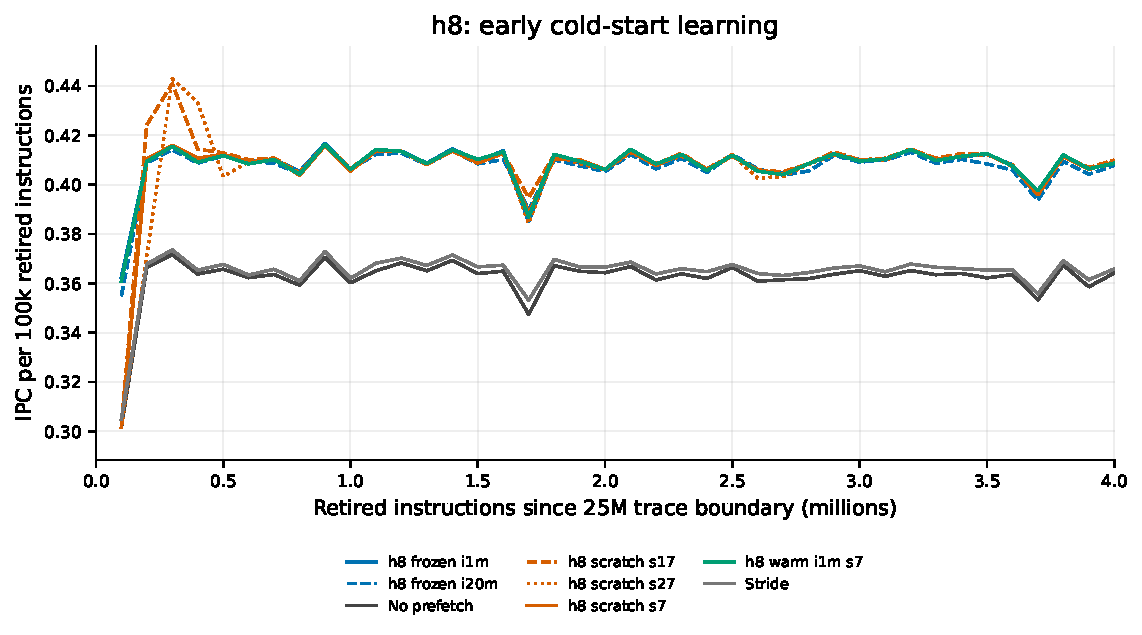
\includegraphics[width=0.92\linewidth]{figures/figure_01_ipc.pdf}
\caption{Early measurements use 100k-instruction intervals. They describe the startup trajectory; the predeclared learning milestones continue to use three consecutive 1M windows.}
\end{figure}

\begin{figure}[p]
\centering
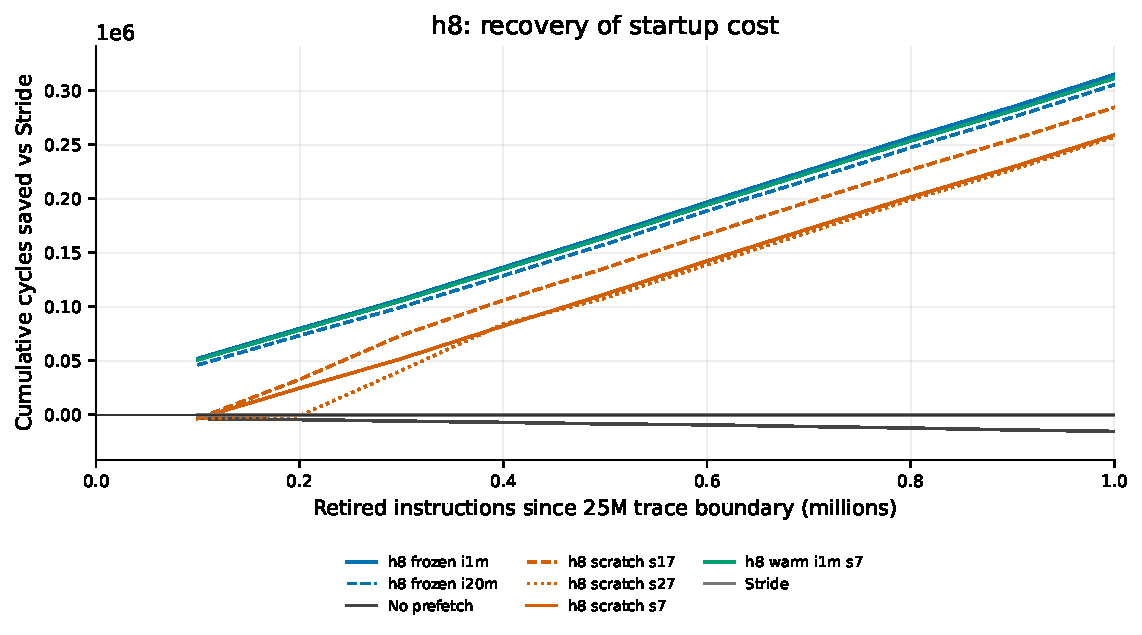
\includegraphics[width=0.92\linewidth]{figures/figure_02_cumulative_cycles_saved_vs_stride.pdf}
\caption{The first million instructions retains the initially negative region. A single positive sampled endpoint is descriptive and does not replace the three-window stability rule.}
\end{figure}

The observed h8 scratch startup samples were at 0.1M: -3,568 saved cycles, 1,659 callbacks, and 25 completed updates; at 0.5M: 107,914--135,701 saved cycles, 8,100 callbacks, and 126 completed updates; at 1M: 257,123--284,360 saved cycles, 16,196 callbacks, and 253 completed updates. These sampled values do not identify an exact event-level crossing time.

\begin{figure}[p]
\centering
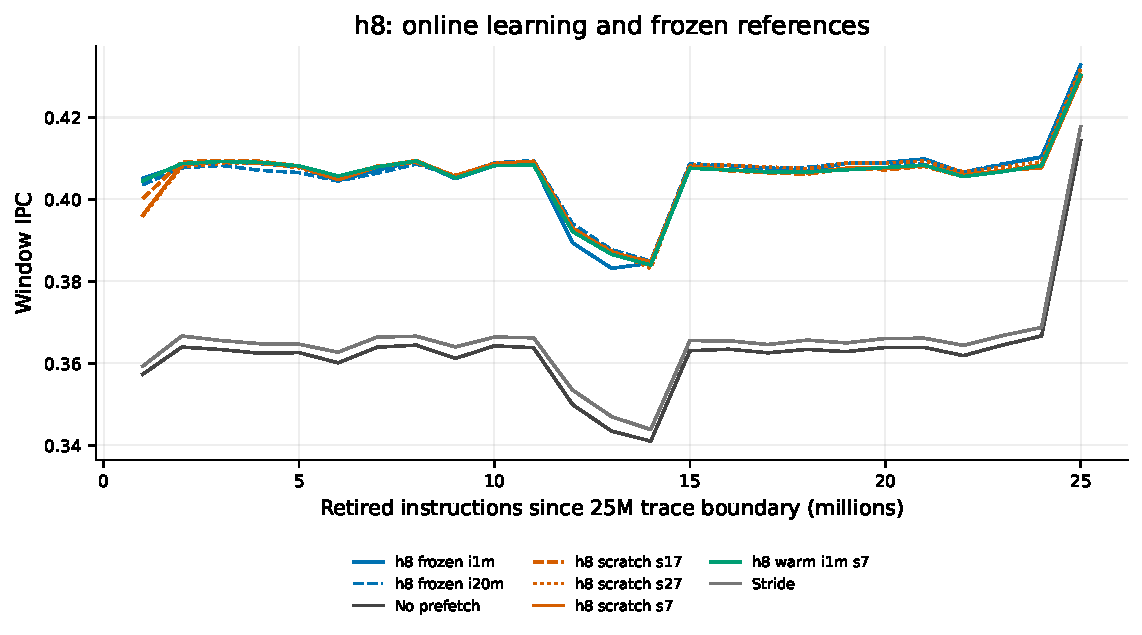
\includegraphics[width=0.92\linewidth]{figures/figure_03_ipc.pdf}
\caption{Cold-start functional measurements. Each point is a 1M-retired-instruction window. Scratch seeds 7, 17, and 27 are separate runs; pretrained checkpoints have only seed 7. Missing or undefined ordinates are not interpolated.}
\end{figure}

\begin{figure}[p]
\centering
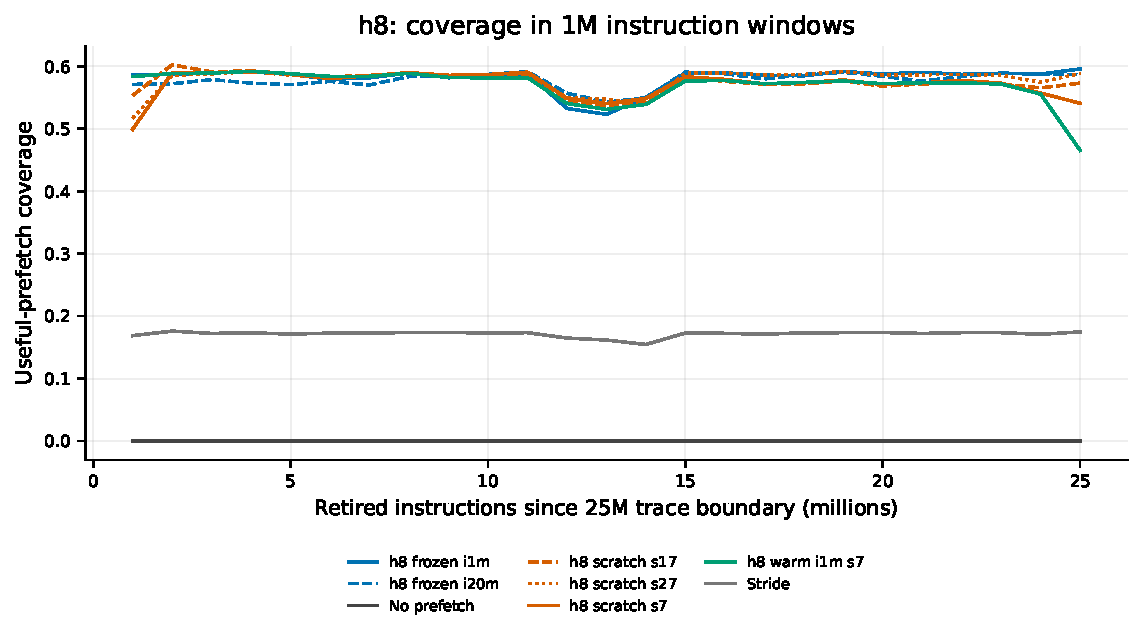
\includegraphics[width=0.92\linewidth]{figures/figure_04_useful_prefetch_coverage.pdf}
\caption{Cold-start functional measurements. Each point is a 1M-retired-instruction window. Scratch seeds 7, 17, and 27 are separate runs; pretrained checkpoints have only seed 7. Missing or undefined ordinates are not interpolated.}
\end{figure}

\begin{figure}[p]
\centering
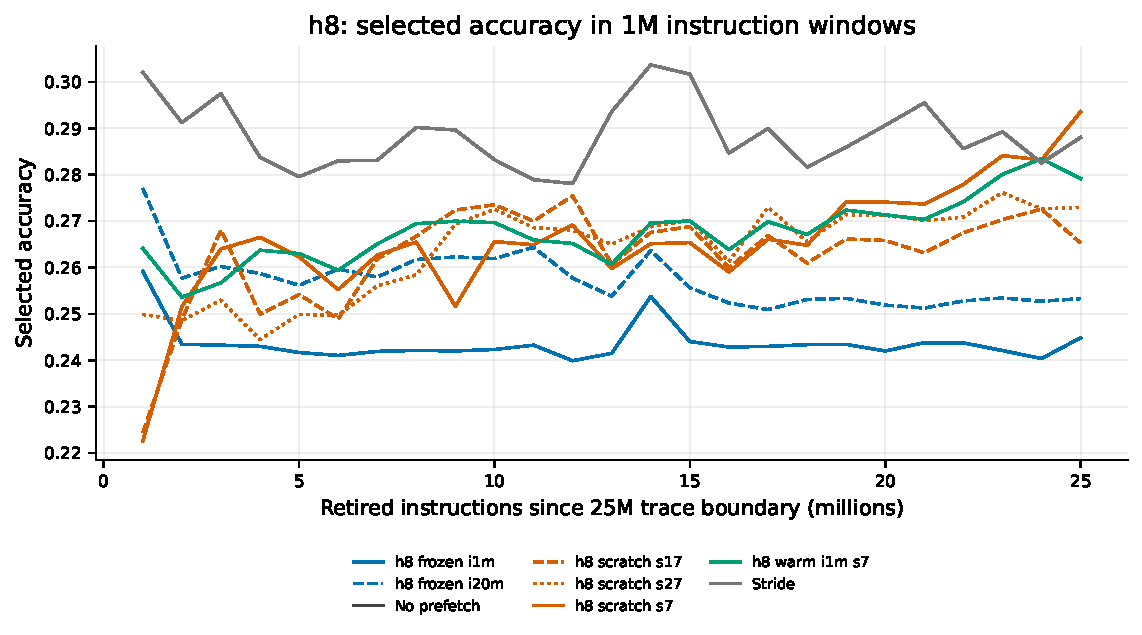
\includegraphics[width=0.92\linewidth]{figures/figure_05_selected_accuracy.pdf}
\caption{Cold-start functional measurements. Each point is a 1M-retired-instruction window. Scratch seeds 7, 17, and 27 are separate runs; pretrained checkpoints have only seed 7. Missing or undefined ordinates are not interpolated.}
\end{figure}

\begin{figure}[p]
\centering
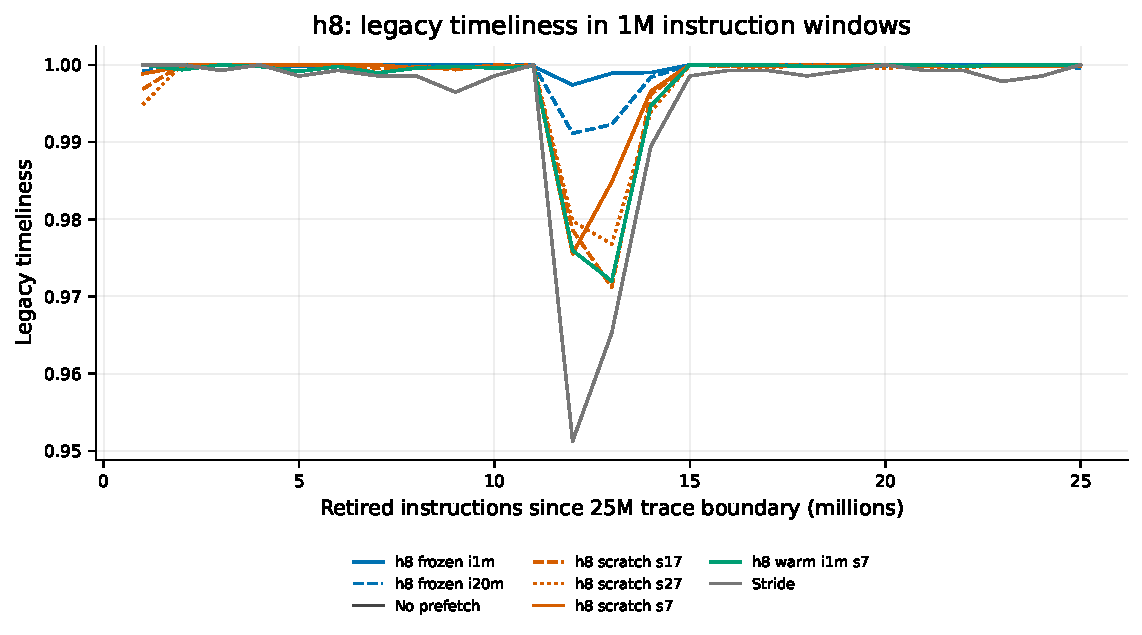
\includegraphics[width=0.92\linewidth]{figures/figure_06_legacy_timeliness.pdf}
\caption{Cold-start functional measurements. Each point is a 1M-retired-instruction window. Scratch seeds 7, 17, and 27 are separate runs; pretrained checkpoints have only seed 7. Missing or undefined ordinates are not interpolated.}
\end{figure}

\begin{figure}[p]
\centering
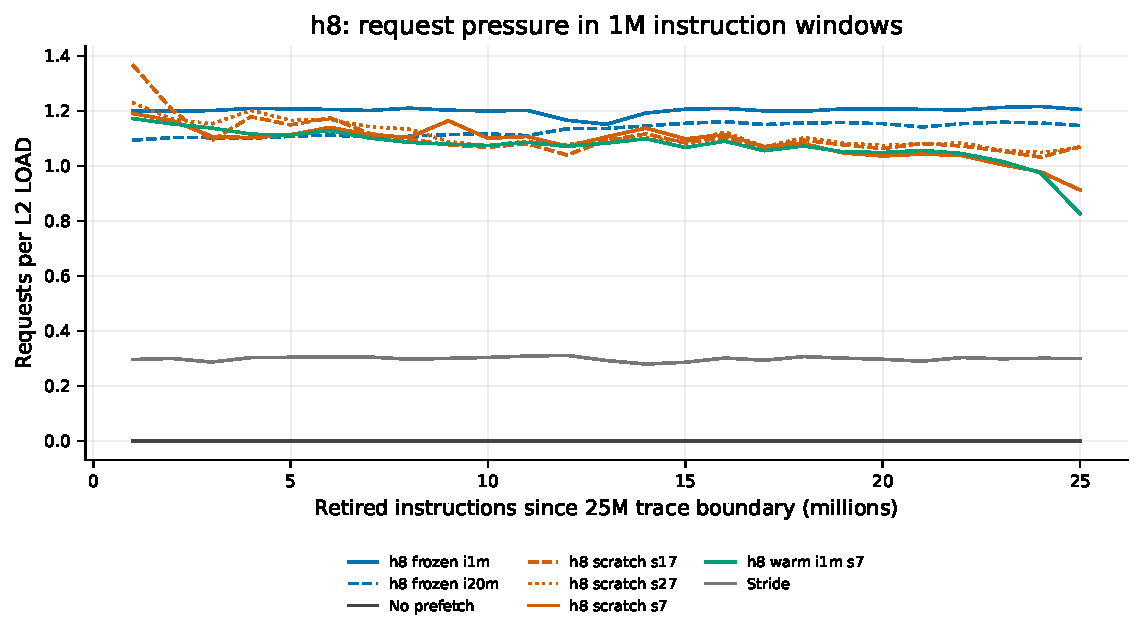
\includegraphics[width=0.92\linewidth]{figures/figure_07_request_pressure.pdf}
\caption{Cold-start functional measurements. Each point is a 1M-retired-instruction window. Scratch seeds 7, 17, and 27 are separate runs; pretrained checkpoints have only seed 7. Missing or undefined ordinates are not interpolated.}
\end{figure}

\begin{figure}[p]
\centering
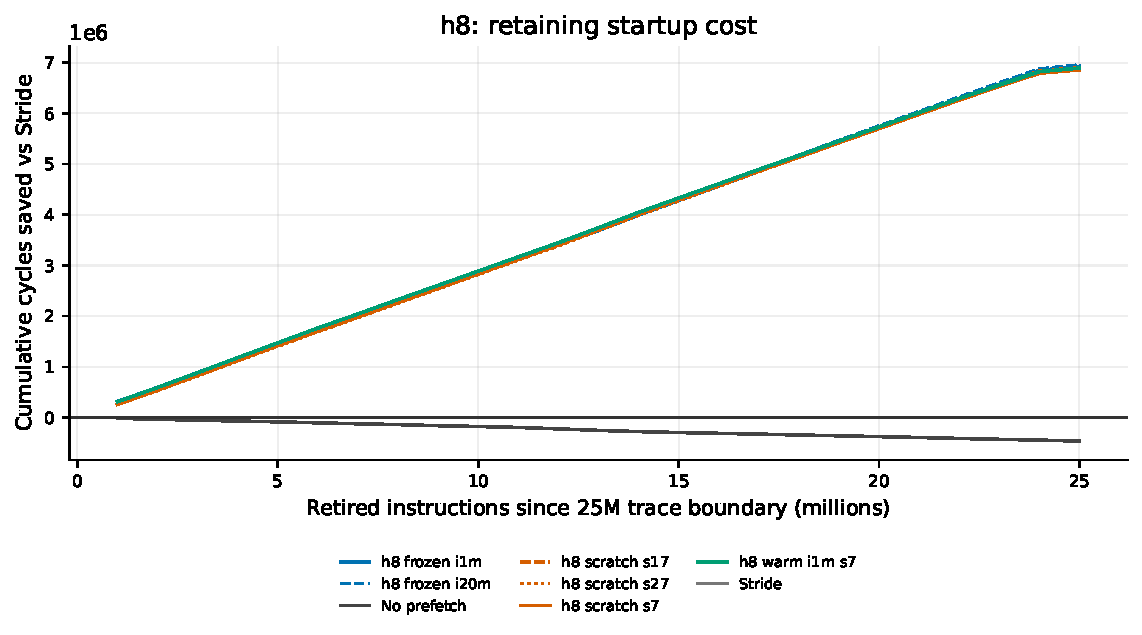
\includegraphics[width=0.92\linewidth]{figures/figure_08_cumulative_cycles_saved_vs_stride.pdf}
\caption{Positive cumulative saving means the run has recovered its startup cost relative to the matched cold-start Stride run. A good late window alone does not establish an end-to-end improvement.}
\end{figure}

\begin{figure}[p]
\centering
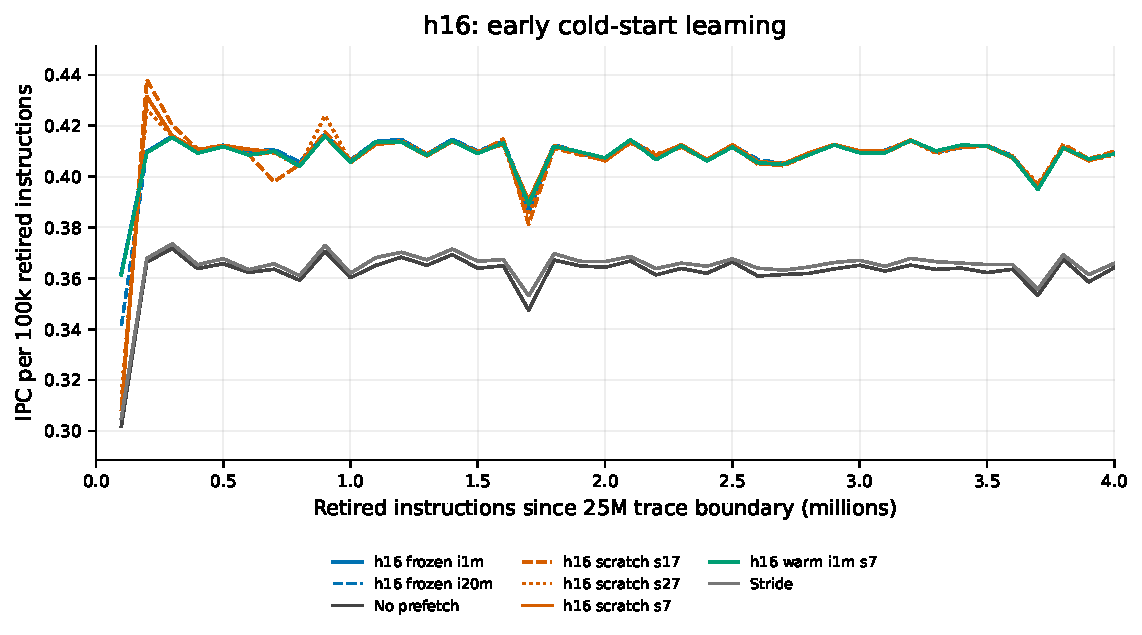
\includegraphics[width=0.92\linewidth]{figures/figure_09_ipc.pdf}
\caption{Early measurements use 100k-instruction intervals. They describe the startup trajectory; the predeclared learning milestones continue to use three consecutive 1M windows.}
\end{figure}

\begin{figure}[p]
\centering
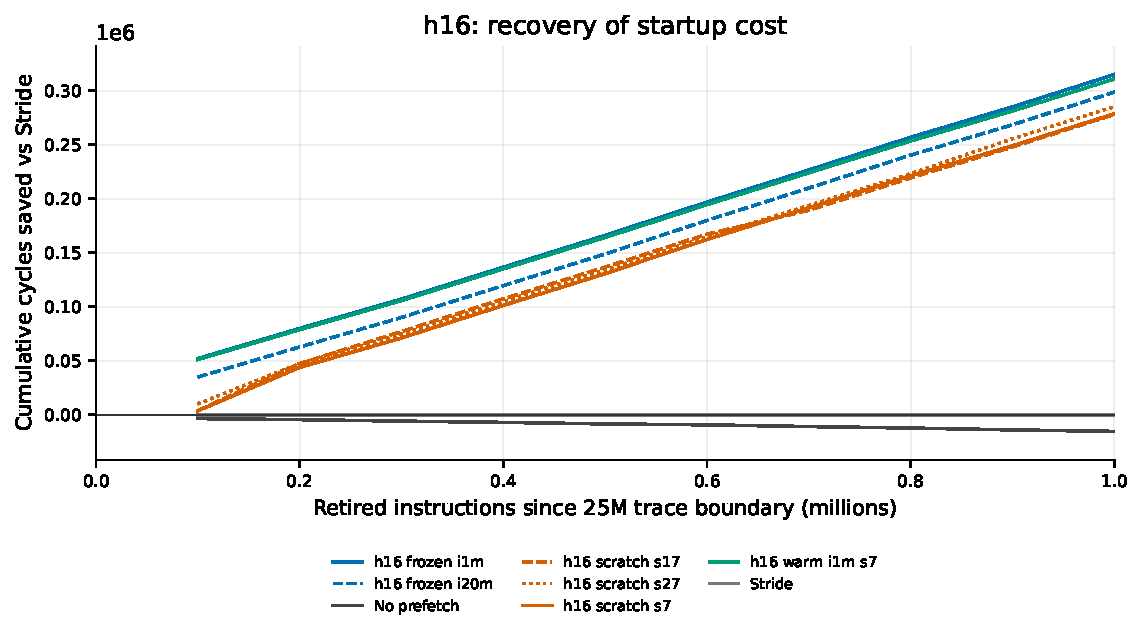
\includegraphics[width=0.92\linewidth]{figures/figure_10_cumulative_cycles_saved_vs_stride.pdf}
\caption{The first million instructions retains the initially negative region. A single positive sampled endpoint is descriptive and does not replace the three-window stability rule.}
\end{figure}

The observed h16 scratch startup samples were at 0.1M: 3,632--10,047 saved cycles, 1,659 callbacks, and 25 completed updates; at 0.5M: 130,587--136,696 saved cycles, 8,100 callbacks, and 126 completed updates; at 1M: 278,070--285,305 saved cycles, 16,196 callbacks, and 253 completed updates. These sampled values do not identify an exact event-level crossing time.

\begin{figure}[p]
\centering
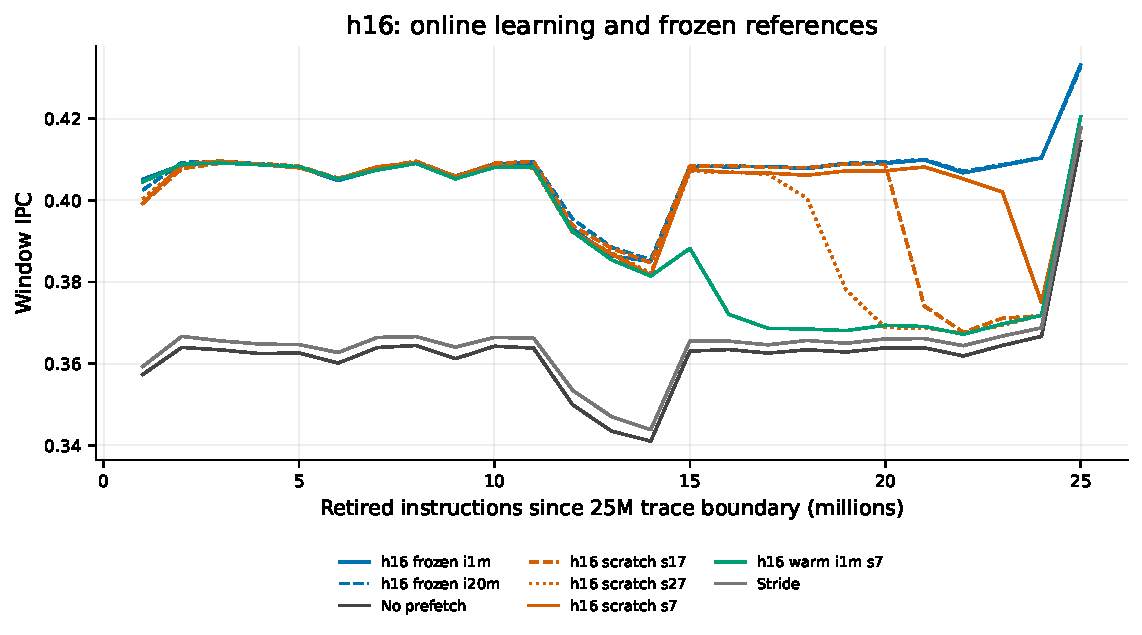
\includegraphics[width=0.92\linewidth]{figures/figure_11_ipc.pdf}
\caption{Cold-start functional measurements. Each point is a 1M-retired-instruction window. Scratch seeds 7, 17, and 27 are separate runs; pretrained checkpoints have only seed 7. Missing or undefined ordinates are not interpolated.}
\end{figure}

\begin{figure}[p]
\centering
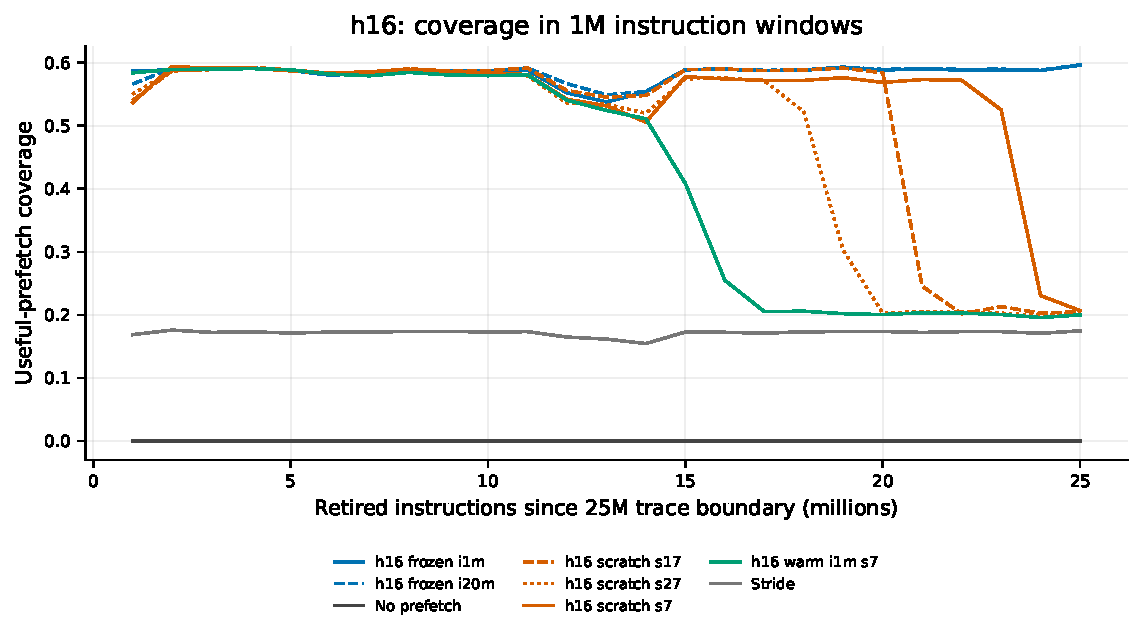
\includegraphics[width=0.92\linewidth]{figures/figure_12_useful_prefetch_coverage.pdf}
\caption{Cold-start functional measurements. Each point is a 1M-retired-instruction window. Scratch seeds 7, 17, and 27 are separate runs; pretrained checkpoints have only seed 7. Missing or undefined ordinates are not interpolated.}
\end{figure}

\begin{figure}[p]
\centering
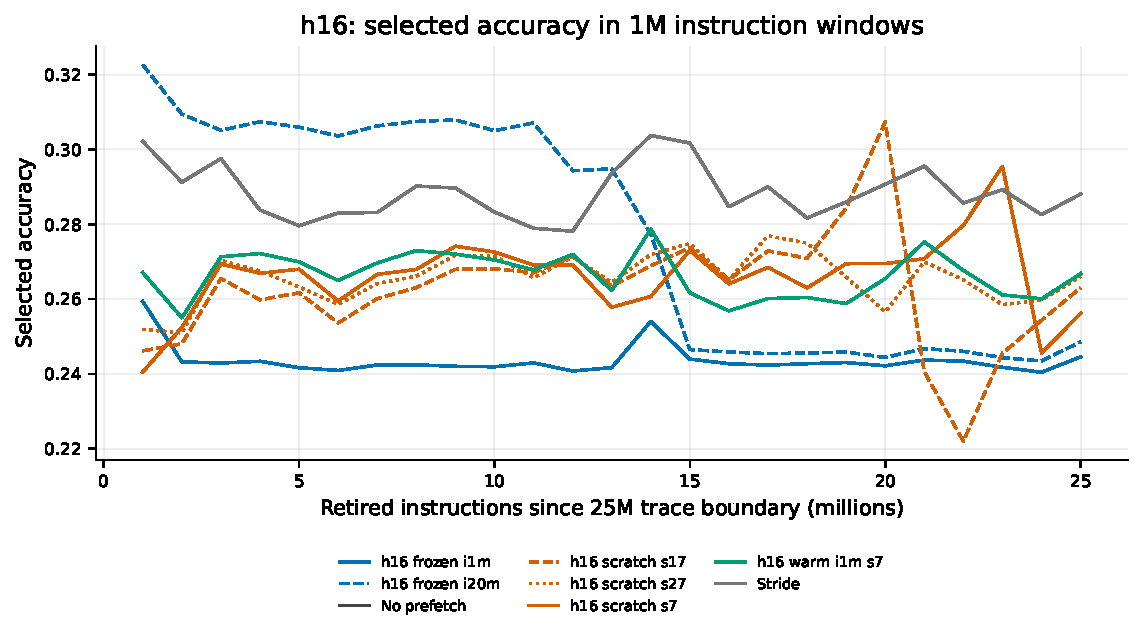
\includegraphics[width=0.92\linewidth]{figures/figure_13_selected_accuracy.pdf}
\caption{Cold-start functional measurements. Each point is a 1M-retired-instruction window. Scratch seeds 7, 17, and 27 are separate runs; pretrained checkpoints have only seed 7. Missing or undefined ordinates are not interpolated.}
\end{figure}

\begin{figure}[p]
\centering
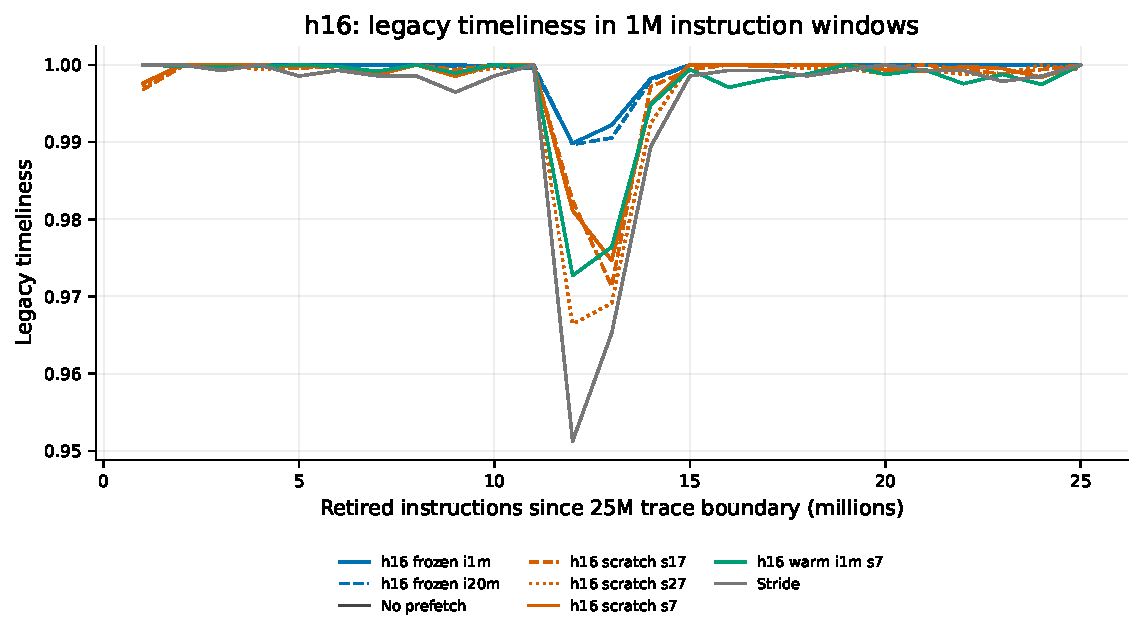
\includegraphics[width=0.92\linewidth]{figures/figure_14_legacy_timeliness.pdf}
\caption{Cold-start functional measurements. Each point is a 1M-retired-instruction window. Scratch seeds 7, 17, and 27 are separate runs; pretrained checkpoints have only seed 7. Missing or undefined ordinates are not interpolated.}
\end{figure}

\begin{figure}[p]
\centering
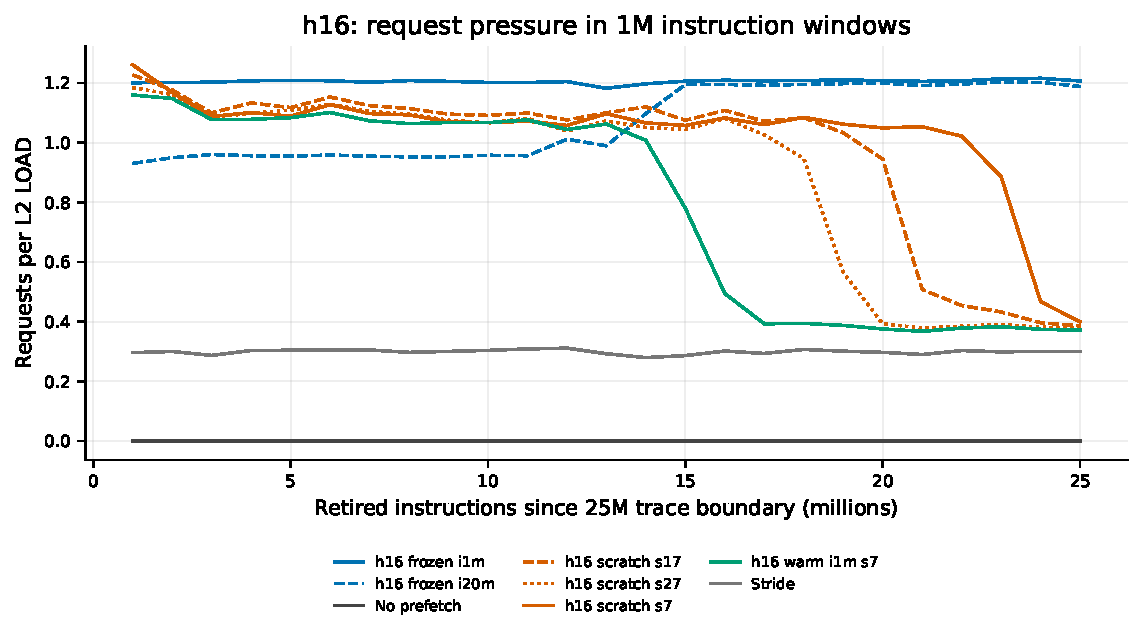
\includegraphics[width=0.92\linewidth]{figures/figure_15_request_pressure.pdf}
\caption{Cold-start functional measurements. Each point is a 1M-retired-instruction window. Scratch seeds 7, 17, and 27 are separate runs; pretrained checkpoints have only seed 7. Missing or undefined ordinates are not interpolated.}
\end{figure}

\begin{figure}[p]
\centering
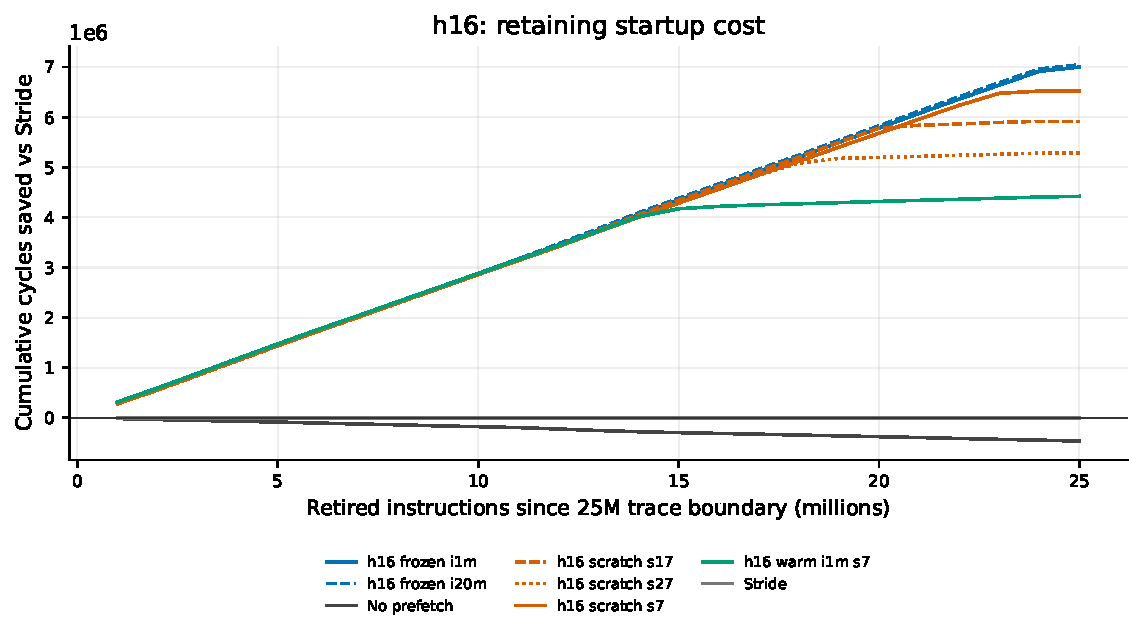
\includegraphics[width=0.92\linewidth]{figures/figure_16_cumulative_cycles_saved_vs_stride.pdf}
\caption{Positive cumulative saving means the run has recovered its startup cost relative to the matched cold-start Stride run. A good late window alone does not establish an end-to-end improvement.}
\end{figure}

\clearpage\section{Observed learning milestones}

The descriptive stability rule is three consecutive 1M-retired-instruction endpoints with positive cumulative cycle savings versus Stride. The separate frozen target requires window IPC at least 99\% of same-H frozen-i1m IPC in three consecutive 1M windows. Tables give the first qualifying window endpoint and the confirmation endpoint. This rule is not an online controller or a statistical equivalence test. Positive window streaks are retained separately in CSV; they do not imply startup has been recovered.

\begin{center}
\scriptsize
\begin{longtable}{llrrrr}
\toprule
Run & Milestone & First M & Confirm M & Updates first/conf. & Callbacks first/conf. \\
\midrule
\endhead
h16 scratch s17 & Saved cycles & 1.0 & 3.0 & 253/757 & 16,196/48,453 \\
h16 scratch s17 & 99\% frozen & 2.0 & 4.0 & 505/1,008 & 32,320/64,553 \\
h16 scratch s27 & Saved cycles & 1.0 & 3.0 & 253/757 & 16,196/48,453 \\
h16 scratch s27 & 99\% frozen & 2.0 & 4.0 & 505/1,008 & 32,320/64,553 \\
h16 scratch s7 & Saved cycles & 1.0 & 3.0 & 253/757 & 16,196/48,453 \\
h16 scratch s7 & 99\% frozen & 2.0 & 4.0 & 505/1,008 & 32,320/64,553 \\
h8 scratch s17 & Saved cycles & 1.0 & 3.0 & 253/757 & 16,196/48,453 \\
h8 scratch s17 & 99\% frozen & 2.0 & 4.0 & 505/1,008 & 32,320/64,553 \\
h8 scratch s27 & Saved cycles & 1.0 & 3.0 & 253/757 & 16,196/48,453 \\
h8 scratch s27 & 99\% frozen & 2.0 & 4.0 & 505/1,008 & 32,320/64,553 \\
h8 scratch s7 & Saved cycles & 1.0 & 3.0 & 253/757 & 16,196/48,453 \\
h8 scratch s7 & 99\% frozen & 2.0 & 4.0 & 505/1,008 & 32,320/64,553 \\
h16 warm i1m s7 & Saved cycles & 1.0 & 3.0 & 253/757 & 16,196/48,453 \\
h16 warm i1m s7 & 99\% frozen & 1.0 & 3.0 & 253/757 & 16,196/48,453 \\
h8 warm i1m s7 & Saved cycles & 1.0 & 3.0 & 253/757 & 16,196/48,453 \\
h8 warm i1m s7 & 99\% frozen & 1.0 & 3.0 & 253/757 & 16,196/48,453 \\
\bottomrule
\end{longtable}
\end{center}

\begin{center}
\scriptsize
\begin{longtable}{llrrrr}
\toprule
Run & Milestone & Coverage & Selected accuracy & Timeliness & $P/N_L$ \\
\midrule
\endhead
h16 scratch s17 & Saved cycles & 0.5398 & 0.2462 & 0.9968 & 1.2275 \\
h16 scratch s17 & 99\% frozen & 0.5875 & 0.2481 & 0.9998 & 1.1773 \\
h16 scratch s27 & Saved cycles & 0.5500 & 0.2519 & 0.9973 & 1.1847 \\
h16 scratch s27 & 99\% frozen & 0.5866 & 0.2509 & 1.0000 & 1.1620 \\
h16 scratch s7 & Saved cycles & 0.5364 & 0.2405 & 0.9976 & 1.2614 \\
h16 scratch s7 & 99\% frozen & 0.5937 & 0.2524 & 1.0000 & 1.1692 \\
h8 scratch s17 & Saved cycles & 0.5531 & 0.2243 & 0.9969 & 1.3675 \\
h8 scratch s17 & 99\% frozen & 0.6022 & 0.2488 & 1.0000 & 1.2033 \\
h8 scratch s27 & Saved cycles & 0.5167 & 0.2499 & 0.9948 & 1.2304 \\
h8 scratch s27 & 99\% frozen & 0.5853 & 0.2485 & 1.0000 & 1.1707 \\
h8 scratch s7 & Saved cycles & 0.4991 & 0.2225 & 0.9988 & 1.1906 \\
h8 scratch s7 & 99\% frozen & 0.5894 & 0.2515 & 0.9998 & 1.1650 \\
h16 warm i1m s7 & Saved cycles & 0.5838 & 0.2670 & 1.0000 & 1.1603 \\
h16 warm i1m s7 & 99\% frozen & 0.5838 & 0.2670 & 1.0000 & 1.1603 \\
h8 warm i1m s7 & Saved cycles & 0.5834 & 0.2641 & 1.0000 & 1.1723 \\
h8 warm i1m s7 & 99\% frozen & 0.5834 & 0.2641 & 1.0000 & 1.1723 \\
\bottomrule
\end{longtable}
\end{center}

The corresponding coverage, selected accuracy, legacy timeliness, request pressure, supervised decisions, exposures, and published versions are in \texttt{learning\_milestones.csv}; they remain separate quantities rather than a composite score.

\section{Cache occupancy, turnover, and lifecycle outcomes}

Occupancy counts simultaneously valid L2 lines. A valid-to-valid replacement changes the resident line without increasing fullness. Demand LOAD, RFO, prefetch, and writeback fills are separate, alongside replacement count and useful-line lifetimes. Fullness is not proof of a warmed working set or a deadline after which prefetching is useless.

The active L2 geometry is 512 sets $\times$ 8 ways $\times$ 64 bytes per line: 4,096 lines, 262,144 bytes (256 KiB).

\begin{figure}[p]
\centering
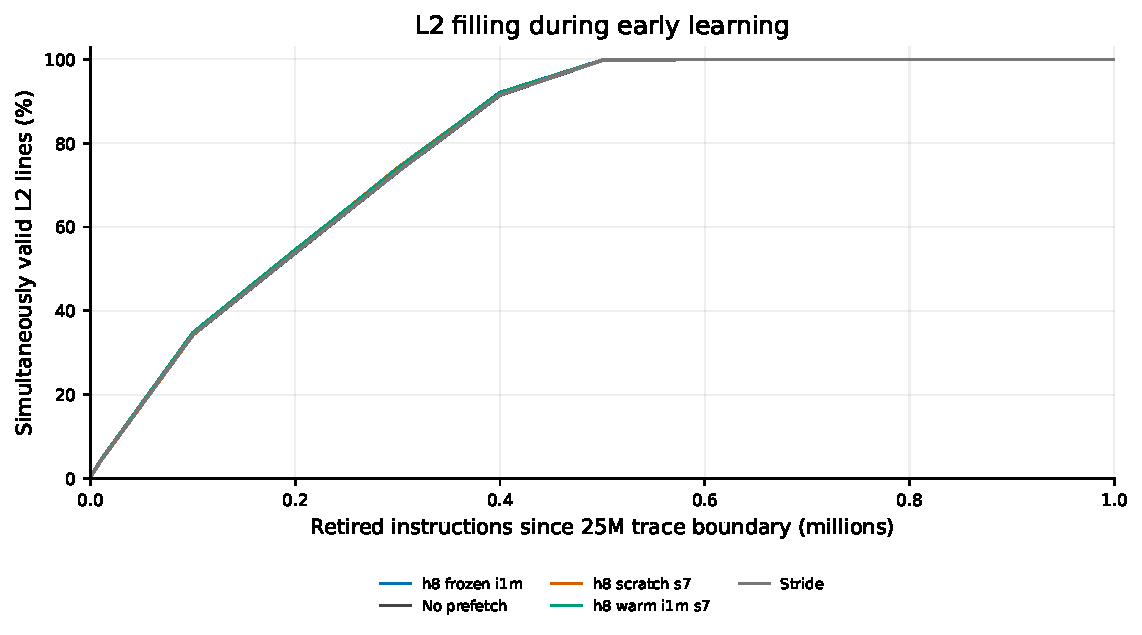
\includegraphics[width=0.92\linewidth]{figures/figure_17_occupancy.pdf}
\caption{The trace-slice origin is 25M target instructions; this plot expands its first million instructions. Exact fill-event first-attainment records, rather than cumulative fill counts, determine the occupancy milestones.}
\end{figure}

\begin{figure}[p]
\centering
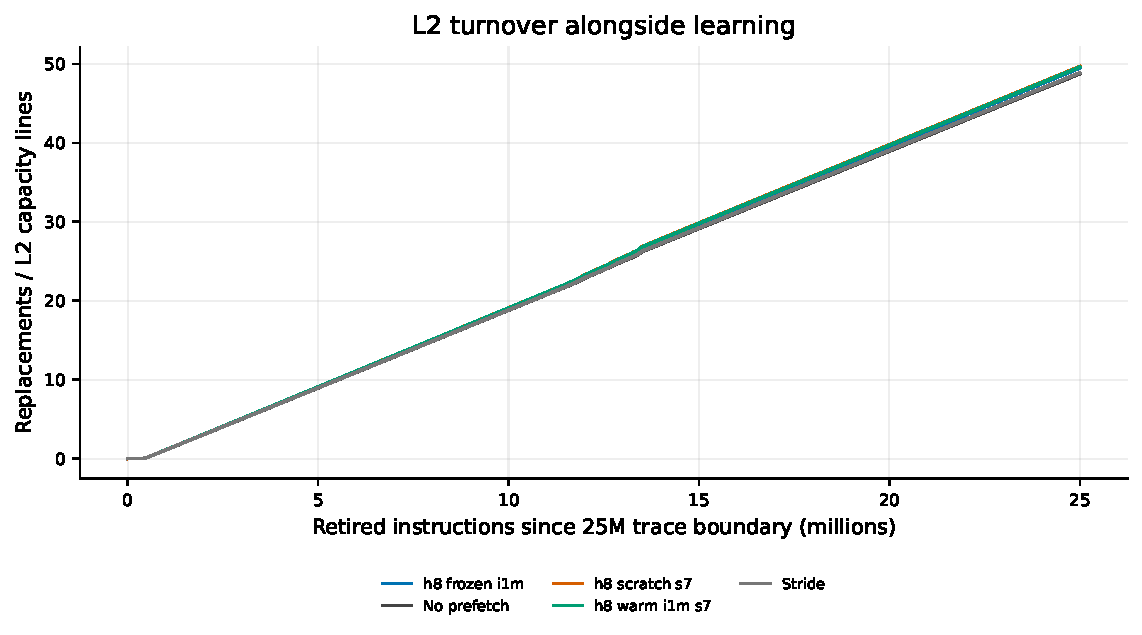
\includegraphics[width=0.92\linewidth]{figures/figure_18_replacement_turnovers.pdf}
\caption{Turnover is cumulative valid-to-valid replacements normalized by actual L2 line capacity. It is distinct from simultaneous occupancy and from useful-prefetch coverage.}
\end{figure}

\begin{figure}[p]
\centering
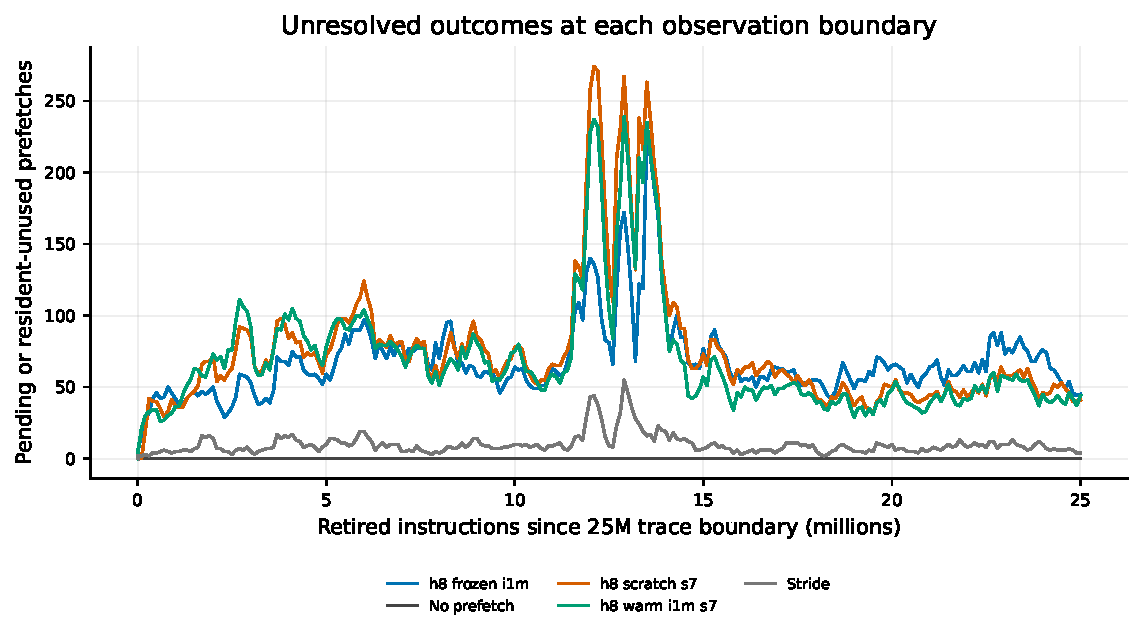
\includegraphics[width=0.92\linewidth]{figures/figure_19_censored_requests.pdf}
\caption{These outcomes remain censored at the displayed boundary. Their later outcomes do not retroactively redefine a window's observed state; final issue-cohort data are provided separately.}
\end{figure}

\begin{center}
\small
\begin{longtable}{lrrr}
\toprule
Run & Occupancy & Instructions & Cycles \\
\midrule
\endhead
h8 frozen i1m & 50\% & 176,919 & 464,590 \\
h8 frozen i1m & 90\% & 388,585 & 977,223 \\
h8 frozen i1m & 95\% & 417,448 & 1,046,864 \\
h8 frozen i1m & 99\% & 460,465 & 1,152,325 \\
h8 frozen i1m & 100\% & 536,006 & 1,334,484 \\
No prefetch & 50\% & 180,391 & 551,809 \\
No prefetch & 90\% & 392,060 & 1,126,716 \\
No prefetch & 95\% & 420,440 & 1,203,868 \\
No prefetch & 99\% & 461,565 & 1,317,623 \\
No prefetch & 100\% & 536,244 & 1,520,774 \\
h8 scratch s7 & 50\% & 178,091 & 523,505 \\
h8 scratch s7 & 90\% & 389,162 & 1,032,946 \\
h8 scratch s7 & 95\% & 418,460 & 1,103,497 \\
h8 scratch s7 & 99\% & 460,685 & 1,207,191 \\
h8 scratch s7 & 100\% & 536,006 & 1,389,058 \\
h8 warm i1m s7 & 50\% & 176,553 & 465,093 \\
h8 warm i1m s7 & 90\% & 389,020 & 980,026 \\
h8 warm i1m s7 & 95\% & 417,660 & 1,049,035 \\
h8 warm i1m s7 & 99\% & 460,625 & 1,154,770 \\
h8 warm i1m s7 & 100\% & 536,006 & 1,336,799 \\
Stride & 50\% & 180,091 & 546,618 \\
Stride & 90\% & 391,562 & 1,118,246 \\
Stride & 95\% & 420,040 & 1,195,372 \\
Stride & 99\% & 461,565 & 1,309,716 \\
Stride & 100\% & 536,244 & 1,512,126 \\
\bottomrule
\end{longtable}
\end{center}

The supplementary \texttt{issue\_cohorts.csv} tracks actual unique PQ enqueues by issue-instruction cohort. Terminal outcomes are timely first demand, late first demand, unused eviction, redundant cache hit, or redundant in-flight request. Pending and resident-unused requests remain censored. These exclusive cohort outcomes are separate from legacy issued/merged counters and are not relabeled as the legacy accuracy or timeliness metrics.

\begin{center}
\scriptsize
\begin{longtable}{lrrrrrr}
\toprule
Run & LOAD fills & RFO fills & PF fills & WB fills & Replacements & Useful lifetimes \\
\midrule
\endhead
h8 frozen i1m & 85,475 & 2 & 121,310 & 0 & 202,691 & 199,717 \\
No prefetch & 203,764 & 2 & 0 & 0 & 199,670 & 199,670 \\
h8 scratch s7 & 87,419 & 2 & 120,129 & 0 & 203,454 & 199,717 \\
h8 warm i1m s7 & 87,778 & 2 & 119,501 & 0 & 203,185 & 199,716 \\
Stride & 168,865 & 2 & 35,439 & 0 & 200,210 & 199,675 \\
\bottomrule
\end{longtable}
\end{center}

\begin{center}
\scriptsize
\begin{longtable}{lrrr}
\toprule
Run & Mean closed line lifetime & Mean useful closed lifetime & Mean PF fill to first use \\
\midrule
\endhead
h8 frozen i1m & 1,142,718.8 & 1,143,143.0 & 3,716.9 \\
No prefetch & 1,303,645.7 & 1,303,645.7 & NA \\
h8 scratch s7 & 1,141,630.2 & 1,141,235.8 & 2,703.7 \\
h8 warm i1m s7 & 1,143,321.8 & 1,143,359.6 & 2,755.2 \\
Stride & 1,291,315.4 & 1,291,631.5 & 1,463.0 \\
\bottomrule
\end{longtable}
\end{center}

Lifetime means are simulated cycles, not fill counts. Closed resident lifetimes end on eviction or invalidation; the useful subset served a demand or RFO at fill or during residence. Prefetch fill-to-first-use measures the first demand on a prefetched line. Still-resident line lifetimes are censored rather than assigned an end time; historical lines whose birth predates measurement have no fabricated start time.

\begin{center}
\scriptsize
\begin{longtable}{llrrrrr}
\toprule
Run & Learning endpoint & M instr. & Occupancy & Replacements & Turnovers & Updates \\
\midrule
\endhead
h16 scratch s17 & Saving first & 1.0 & 100.0\% & 4,581 & 1.12 & 253 \\
h16 scratch s17 & Saving confirm & 3.0 & 100.0\% & 20,731 & 5.06 & 757 \\
h16 scratch s17 & 99\% frozen first & 2.0 & 100.0\% & 12,649 & 3.09 & 505 \\
h16 scratch s17 & 99\% frozen confirm & 4.0 & 100.0\% & 28,835 & 7.04 & 1,008 \\
h16 scratch s27 & Saving first & 1.0 & 100.0\% & 4,576 & 1.12 & 253 \\
h16 scratch s27 & Saving confirm & 3.0 & 100.0\% & 20,754 & 5.07 & 757 \\
h16 scratch s27 & 99\% frozen first & 2.0 & 100.0\% & 12,654 & 3.09 & 505 \\
h16 scratch s27 & 99\% frozen confirm & 4.0 & 100.0\% & 28,872 & 7.05 & 1,008 \\
h16 scratch s7 & Saving first & 1.0 & 100.0\% & 4,576 & 1.12 & 253 \\
h16 scratch s7 & Saving confirm & 3.0 & 100.0\% & 20,796 & 5.08 & 757 \\
h16 scratch s7 & 99\% frozen first & 2.0 & 100.0\% & 12,671 & 3.09 & 505 \\
h16 scratch s7 & 99\% frozen confirm & 4.0 & 100.0\% & 28,926 & 7.06 & 1,008 \\
h8 scratch s17 & Saving first & 1.0 & 100.0\% & 4,580 & 1.12 & 253 \\
h8 scratch s17 & Saving confirm & 3.0 & 100.0\% & 20,814 & 5.08 & 757 \\
h8 scratch s17 & 99\% frozen first & 2.0 & 100.0\% & 12,670 & 3.09 & 505 \\
h8 scratch s17 & 99\% frozen confirm & 4.0 & 100.0\% & 28,936 & 7.06 & 1,008 \\
h8 scratch s27 & Saving first & 1.0 & 100.0\% & 4,553 & 1.11 & 253 \\
h8 scratch s27 & Saving confirm & 3.0 & 100.0\% & 20,670 & 5.05 & 757 \\
h8 scratch s27 & 99\% frozen first & 2.0 & 100.0\% & 12,605 & 3.08 & 505 \\
h8 scratch s27 & 99\% frozen confirm & 4.0 & 100.0\% & 28,766 & 7.02 & 1,008 \\
h8 scratch s7 & Saving first & 1.0 & 100.0\% & 4,560 & 1.11 & 253 \\
h8 scratch s7 & Saving confirm & 3.0 & 100.0\% & 20,795 & 5.08 & 757 \\
h8 scratch s7 & 99\% frozen first & 2.0 & 100.0\% & 12,665 & 3.09 & 505 \\
h8 scratch s7 & 99\% frozen confirm & 4.0 & 100.0\% & 28,915 & 7.06 & 1,008 \\
h16 warm i1m s7 & Saving first & 1.0 & 100.0\% & 4,558 & 1.11 & 253 \\
h16 warm i1m s7 & Saving confirm & 3.0 & 100.0\% & 20,797 & 5.08 & 757 \\
h16 warm i1m s7 & 99\% frozen first & 1.0 & 100.0\% & 4,558 & 1.11 & 253 \\
h16 warm i1m s7 & 99\% frozen confirm & 3.0 & 100.0\% & 20,797 & 5.08 & 757 \\
h8 warm i1m s7 & Saving first & 1.0 & 100.0\% & 4,562 & 1.11 & 253 \\
h8 warm i1m s7 & Saving confirm & 3.0 & 100.0\% & 20,830 & 5.09 & 757 \\
h8 warm i1m s7 & 99\% frozen first & 1.0 & 100.0\% & 4,562 & 1.11 & 253 \\
h8 warm i1m s7 & 99\% frozen confirm & 3.0 & 100.0\% & 20,830 & 5.09 & 757 \\
\bottomrule
\end{longtable}
\end{center}

The table places cache turnover beside each first and confirmed learning endpoint. A full cache continues replacing lines while learning and useful prefetching continue. Occupancy is neither a working-set warmness test nor a learning deadline.

\clearpage\section{Storage and timing sensitivity}

Unbounded state and zero modeled latency are algorithmic controls. Finite arms use the same exact-PC table and queue limits for frozen and online inference. Equal entry counts do not imply equal byte cost. FP32 weights are 7,632 bytes (7.453 KiB) for h8 and 20,880 bytes (20.391 KiB) for h16. A bare h/c pair requires $8H$ bytes per entry before tags and replacement metadata; a 64-entry table therefore uses 4,096 or 8,192 h/c bytes. No quantized-model measurement is claimed.

The finite-resource sensitivity cases are architectural assumptions, not measured silicon latency, area, power, frequency, or PPA. Inference work depends on the actual model and decoded $K$. Training, active/training weight copies, optimizer moments, publication/copy work, queues, and the shadow teacher must be counted. Host CPU time is not converted into simulated stall cycles. Simulator/CPU co-simulation is not completed on-chip training hardware.

\subsection{Predeclared architectural cost assumptions}

There are separate serial inference and training engines. The two finite cases provide $b\in\{4,16\}$ MACs/cycle with matched weight bandwidth $4b\in\{16,64\}$ bytes/cycle. Each engine has one nonlinear unit at four cycles per operation. Dense, nonlinear, and control phases serialize conservatively. The matched weight-read bandwidth supplies one FP32 weight operand per MAC concurrently within the dense phase; it is not a second serialized full-weight-read charge. The additional bandwidth term below counts scratch/state traffic. The effective inference initiation interval equals its service occupancy because there is one inference in flight; the input queue has 16 entries, output queue 32 addresses, and output issue bandwidth one request/cycle. The learned positive count is not clamped to Stride's degree: the separate 32-address decoder resource bound drops excess output explicitly.

Let $E$ denote the learned positive hurdle and $K$ the actually decoded count after explicit resource limits. Inference work is

\[F_{\rm infer}=128H+8H^2+2H+EH+K(3H^2+4H),\qquad Z_{\rm infer}=6H+E+K(3H+1).\]

Its service time is $\lceil F_{\rm infer}/b\rceil+4Z_{\rm infer}+8+\lceil S/4\rceil+4K+\lceil T_{\rm infer}/(4b)\rceil$, where $S$ is live state entries and $T_{\rm infer}=4(128+4H)+24K$ bytes accounts for scratch/state/output traffic. This is a sensitivity model, not a measured pipeline.

For each 64-decision batch, $R$ is actual padded projection positions, $n_+$ the number of positive decisions, and $A$ the teacher action count. $P_\theta=11H^2+150H+4$ is parameter count. The actual forward MAC estimate and conservative backward/optimizer costs are

\[F_{\rm train}=128HR+64(8H^2+2H)+n_+H+A(3H^2+4H),\]

\[Z_{\rm train}=RH+320H+3AH+192+n_++2P_\theta.\]

Training costs $\lceil3F_{\rm train}/b\rceil+12Z_{\rm train}+512+12P_\theta+\lceil T_{\rm train}/(4b)\rceil$ cycles, with $T_{\rm train}=32P_\theta+4(128R+128H+AH)$ bytes. The backward MAC bound is twice forward, so total modeled forward/backward work is three times forward; it is not a profiler measurement of PyTorch kernels. Adam/state movement and parameter copying are counted separately. Publication costs $\lceil4P_\theta/(4b)\rceil+8$ cycles. One update may be in flight and 64 additional decisions pending; a full pending queue drops training admission explicitly.

The shadow teacher assumes a separate 24-stage, initiation-interval-one pipeline: four tag comparators in each of 16 stages (64 comparator lanes across the pipeline), then eight control stages, with distributed stage-local tag reads, ideal tracker-state forwarding and a 64-entry label queue. The active L2 accepts at most one read per cycle, so its actual eligible callbacks respect this input rate. A single unpipelined four-comparator unit would not provide this throughput. Teacher actions become training-available at modeled completion. Parameter publication is coherent, and h/c state becomes available on scheduled inference completion. Pending work is serviced at scheduled simulator cycles even without a new demand callback. The conventional Stride comparator retains its original callback-time requests with no added modeled lookup delay. The finite sensitivity adds service costs to the neural inference and online update engines; it does not retrofit a Stride timing model. The zero-cost controls set modeled service/publication delays to zero while retaining actual CPU co-simulation work.

\begin{center}
\scriptsize
\begin{longtable}{lrrrr}
\toprule
Design & Inference max KiB & Learning max KiB & Inference peaks KiB & Learning peaks KiB \\
\midrule
\endhead
h16 frozen i1m & NA & 0.00 & 37.08 & 0.00 \\
h8 frozen i1m & NA & 0.00 & 17.58 & 0.00 \\
h8 frozen i1m /64 /MAC0 & 16.95 & 0.00 & 14.95 & 0.00 \\
h8 frozen i1m /64 /MAC16 & 16.95 & 0.00 & 15.68 & 0.00 \\
h8 frozen i1m /64 /MAC4 & 16.95 & 0.00 & 15.12 & 0.00 \\
h16 scratch s7 & NA & 2,722.53 & 37.12 & 515.28 \\
h8 scratch s7 & NA & 1,625.84 & 17.58 & 397.72 \\
h8 scratch s7 /64 /MAC0 & 16.95 & 1,625.84 & 14.95 & 397.72 \\
h8 scratch s7 /64 /MAC16 & 16.95 & 1,633.30 & 15.59 & 338.62 \\
h8 scratch s7 /64 /MAC4 & 16.95 & 1,633.30 & 14.93 & 341.10 \\
\bottomrule
\end{longtable}
\end{center}

Inference includes active weights, PC state, arithmetic scratch, active event/result payloads, and input/output queues. The learning subtotal adds the shadow teacher and its queue, examples, padded tensors, TBPTT activations, gradients, optimizer, training weights, publication buffer, and retained version bank. The zero-service unbounded rows have no finite inference maximum; measured occupied-state bytes remain in their peak envelope. The 64-entry rows provide the finite configured total. These are FP32 logical storage costs, not host RSS.

The category table groups runs with the same arm, hidden size, capacity and service case; its observed column takes the maximum across completed seeds/checkpoint budgets within that design. The following per-run totals keep runs separate.

\begin{center}
\scriptsize
\begin{longtable}{p{0.24\linewidth}p{0.43\linewidth}rr}
\toprule
Design & Storage category & Max (B) & Peak (B) \\
\midrule
\endhead
h16 frozen & active FP32 weights & 20,880 & 20,880 \\
h16 frozen & PC tags, valid/replacement metadata and h/c & NA & 14,720 \\
h16 frozen & inference scratch & 2,176 & 2,176 \\
h16 frozen & active event metadata & 56 & 56 \\
h16 frozen & decoded delta/address result payload & 512 & 32 \\
h16 frozen & input queue & 896 & 56 \\
h16 frozen & output queue & 768 & 48 \\
h16 frozen & shadow Stride / conventional Stride state & 0 & 0 \\
h16 frozen & teacher label availability queue & 0 & 0 \\
h8 frozen & active FP32 weights & 7,632 & 7,632 \\
h8 frozen & PC tags, valid/replacement metadata and h/c & NA & 8,832 \\
h8 frozen & inference scratch & 1,344 & 1,344 \\
h8 frozen & active event metadata & 56 & 56 \\
h8 frozen & decoded delta/address result payload & 512 & 32 \\
h8 frozen & input queue & 896 & 56 \\
h8 frozen & output queue & 768 & 48 \\
h8 frozen & shadow Stride / conventional Stride state & 0 & 0 \\
h8 frozen & teacher label availability queue & 0 & 0 \\
h8 frozen /64 /MAC0 & active FP32 weights & 7,632 & 7,632 \\
h8 frozen /64 /MAC0 & PC tags, valid/replacement metadata and h/c & 6,144 & 6,144 \\
h8 frozen /64 /MAC0 & inference scratch & 1,344 & 1,344 \\
h8 frozen /64 /MAC0 & active event metadata & 56 & 56 \\
h8 frozen /64 /MAC0 & decoded delta/address result payload & 512 & 32 \\
h8 frozen /64 /MAC0 & input queue & 896 & 56 \\
h8 frozen /64 /MAC0 & output queue & 768 & 48 \\
h8 frozen /64 /MAC0 & shadow Stride / conventional Stride state & 0 & 0 \\
h8 frozen /64 /MAC0 & teacher label availability queue & 0 & 0 \\
h8 frozen /64 /MAC16 & active FP32 weights & 7,632 & 7,632 \\
h8 frozen /64 /MAC16 & PC tags, valid/replacement metadata and h/c & 6,144 & 6,048 \\
h8 frozen /64 /MAC16 & inference scratch & 1,344 & 1,344 \\
h8 frozen /64 /MAC16 & active event metadata & 56 & 56 \\
h8 frozen /64 /MAC16 & decoded delta/address result payload & 512 & 32 \\
h8 frozen /64 /MAC16 & input queue & 896 & 896 \\
h8 frozen /64 /MAC16 & output queue & 768 & 48 \\
h8 frozen /64 /MAC16 & shadow Stride / conventional Stride state & 0 & 0 \\
h8 frozen /64 /MAC16 & teacher label availability queue & 0 & 0 \\
h8 frozen /64 /MAC4 & active FP32 weights & 7,632 & 7,632 \\
h8 frozen /64 /MAC4 & PC tags, valid/replacement metadata and h/c & 6,144 & 5,472 \\
h8 frozen /64 /MAC4 & inference scratch & 1,344 & 1,344 \\
h8 frozen /64 /MAC4 & active event metadata & 56 & 56 \\
h8 frozen /64 /MAC4 & decoded delta/address result payload & 512 & 32 \\
h8 frozen /64 /MAC4 & input queue & 896 & 896 \\
h8 frozen /64 /MAC4 & output queue & 768 & 48 \\
h8 frozen /64 /MAC4 & shadow Stride / conventional Stride state & 0 & 0 \\
h8 frozen /64 /MAC4 & teacher label availability queue & 0 & 0 \\
No prefetch & active FP32 weights & 0 & 0 \\
No prefetch & PC tags, valid/replacement metadata and h/c & 0 & 0 \\
No prefetch & inference scratch & 0 & 0 \\
No prefetch & active event metadata & 0 & 0 \\
No prefetch & decoded delta/address result payload & 0 & 0 \\
No prefetch & input queue & 0 & 0 \\
No prefetch & output queue & 0 & 0 \\
No prefetch & shadow Stride / conventional Stride state & 0 & 0 \\
No prefetch & teacher label availability queue & 0 & 0 \\
h16 scratch & active FP32 weights & 20,880 & 20,880 \\
h16 scratch & PC tags, valid/replacement metadata and h/c & NA & 14,720 \\
h16 scratch & inference scratch & 2,176 & 2,176 \\
h16 scratch & active event metadata & 56 & 56 \\
h16 scratch & decoded delta/address result payload & 512 & 48 \\
h16 scratch & input queue & 896 & 56 \\
h16 scratch & output queue & 768 & 72 \\
h16 scratch & shadow Stride / conventional Stride state & 2,064 & 2,064 \\
h16 scratch & teacher label availability queue & 3,072 & 48 \\
h16 scratch & bounded training examples and saved start states & 23,552 & 22,528 \\
h16 scratch & padded training input and target tensors & 557,568 & 304,128 \\
h16 scratch & TBPTT autograd-saved activations & 2,097,152 & 94,416 \\
h16 scratch & gradient tensors & 20,880 & 20,880 \\
h16 scratch & Adam moments and step tensors & 41,824 & 41,824 \\
h16 scratch & training FP32 weight copy & 20,880 & 20,880 \\
h16 scratch & publication buffer & 20,880 & 20,880 \\
h16 scratch & retained old inference weight bank & 0 & 0 \\
h8 scratch & active FP32 weights & 7,632 & 7,632 \\
h8 scratch & PC tags, valid/replacement metadata and h/c & NA & 8,832 \\
h8 scratch & inference scratch & 1,344 & 1,344 \\
h8 scratch & active event metadata & 56 & 56 \\
h8 scratch & decoded delta/address result payload & 512 & 48 \\
h8 scratch & input queue & 896 & 56 \\
h8 scratch & output queue & 768 & 72 \\
h8 scratch & shadow Stride / conventional Stride state & 2,064 & 2,064 \\
h8 scratch & teacher label availability queue & 3,072 & 48 \\
h8 scratch & bounded training examples and saved start states & 15,360 & 14,336 \\
h8 scratch & padded training input and target tensors & 557,568 & 304,128 \\
h8 scratch & TBPTT autograd-saved activations & 1,048,576 & 48,464 \\
h8 scratch & gradient tensors & 7,632 & 7,632 \\
h8 scratch & Adam moments and step tensors & 15,328 & 15,328 \\
h8 scratch & training FP32 weight copy & 7,632 & 7,632 \\
h8 scratch & publication buffer & 7,632 & 7,632 \\
h8 scratch & retained old inference weight bank & 0 & 0 \\
h8 scratch /64 /MAC0 & active FP32 weights & 7,632 & 7,632 \\
h8 scratch /64 /MAC0 & PC tags, valid/replacement metadata and h/c & 6,144 & 6,144 \\
h8 scratch /64 /MAC0 & inference scratch & 1,344 & 1,344 \\
h8 scratch /64 /MAC0 & active event metadata & 56 & 56 \\
h8 scratch /64 /MAC0 & decoded delta/address result payload & 512 & 32 \\
h8 scratch /64 /MAC0 & input queue & 896 & 56 \\
h8 scratch /64 /MAC0 & output queue & 768 & 48 \\
h8 scratch /64 /MAC0 & shadow Stride / conventional Stride state & 2,064 & 2,064 \\
h8 scratch /64 /MAC0 & teacher label availability queue & 3,072 & 48 \\
h8 scratch /64 /MAC0 & bounded training examples and saved start states & 15,360 & 14,336 \\
h8 scratch /64 /MAC0 & padded training input and target tensors & 557,568 & 304,128 \\
h8 scratch /64 /MAC0 & TBPTT autograd-saved activations & 1,048,576 & 48,464 \\
h8 scratch /64 /MAC0 & gradient tensors & 7,632 & 7,632 \\
h8 scratch /64 /MAC0 & Adam moments and step tensors & 15,328 & 15,328 \\
h8 scratch /64 /MAC0 & training FP32 weight copy & 7,632 & 7,632 \\
h8 scratch /64 /MAC0 & publication buffer & 7,632 & 7,632 \\
h8 scratch /64 /MAC0 & retained old inference weight bank & 0 & 0 \\
h8 scratch /64 /MAC16 & active FP32 weights & 7,632 & 7,632 \\
h8 scratch /64 /MAC16 & PC tags, valid/replacement metadata and h/c & 6,144 & 5,952 \\
h8 scratch /64 /MAC16 & inference scratch & 1,344 & 1,344 \\
h8 scratch /64 /MAC16 & active event metadata & 56 & 56 \\
h8 scratch /64 /MAC16 & decoded delta/address result payload & 512 & 32 \\
h8 scratch /64 /MAC16 & input queue & 896 & 896 \\
h8 scratch /64 /MAC16 & output queue & 768 & 48 \\
h8 scratch /64 /MAC16 & shadow Stride / conventional Stride state & 2,064 & 2,064 \\
h8 scratch /64 /MAC16 & teacher label availability queue & 3,072 & 336 \\
h8 scratch /64 /MAC16 & bounded training examples and saved start states & 15,360 & 14,240 \\
h8 scratch /64 /MAC16 & padded training input and target tensors & 557,568 & 236,544 \\
h8 scratch /64 /MAC16 & TBPTT autograd-saved activations & 1,048,576 & 47,712 \\
h8 scratch /64 /MAC16 & gradient tensors & 7,632 & 7,632 \\
h8 scratch /64 /MAC16 & Adam moments and step tensors & 15,328 & 15,328 \\
h8 scratch /64 /MAC16 & training FP32 weight copy & 7,632 & 7,632 \\
h8 scratch /64 /MAC16 & publication buffer & 7,632 & 7,632 \\
h8 scratch /64 /MAC16 & retained old inference weight bank & 7,632 & 7,632 \\
h8 scratch /64 /MAC4 & active FP32 weights & 7,632 & 7,632 \\
h8 scratch /64 /MAC4 & PC tags, valid/replacement metadata and h/c & 6,144 & 5,280 \\
h8 scratch /64 /MAC4 & inference scratch & 1,344 & 1,344 \\
h8 scratch /64 /MAC4 & active event metadata & 56 & 56 \\
h8 scratch /64 /MAC4 & decoded delta/address result payload & 512 & 32 \\
h8 scratch /64 /MAC4 & input queue & 896 & 896 \\
h8 scratch /64 /MAC4 & output queue & 768 & 48 \\
h8 scratch /64 /MAC4 & shadow Stride / conventional Stride state & 2,064 & 2,064 \\
h8 scratch /64 /MAC4 & teacher label availability queue & 3,072 & 336 \\
h8 scratch /64 /MAC4 & bounded training examples and saved start states & 15,360 & 14,144 \\
h8 scratch /64 /MAC4 & padded training input and target tensors & 557,568 & 247,104 \\
h8 scratch /64 /MAC4 & TBPTT autograd-saved activations & 1,048,576 & 39,780 \\
h8 scratch /64 /MAC4 & gradient tensors & 7,632 & 7,632 \\
h8 scratch /64 /MAC4 & Adam moments and step tensors & 15,328 & 15,328 \\
h8 scratch /64 /MAC4 & training FP32 weight copy & 7,632 & 7,632 \\
h8 scratch /64 /MAC4 & publication buffer & 7,632 & 7,632 \\
h8 scratch /64 /MAC4 & retained old inference weight bank & 7,632 & 7,632 \\
h16 warm i1m & active FP32 weights & 20,880 & 20,880 \\
h16 warm i1m & PC tags, valid/replacement metadata and h/c & NA & 14,720 \\
h16 warm i1m & inference scratch & 2,176 & 2,176 \\
h16 warm i1m & active event metadata & 56 & 56 \\
h16 warm i1m & decoded delta/address result payload & 512 & 48 \\
h16 warm i1m & input queue & 896 & 56 \\
h16 warm i1m & output queue & 768 & 72 \\
h16 warm i1m & shadow Stride / conventional Stride state & 2,064 & 2,064 \\
h16 warm i1m & teacher label availability queue & 3,072 & 48 \\
h16 warm i1m & bounded training examples and saved start states & 23,552 & 22,528 \\
h16 warm i1m & padded training input and target tensors & 557,568 & 304,128 \\
h16 warm i1m & TBPTT autograd-saved activations & 2,097,152 & 94,416 \\
h16 warm i1m & gradient tensors & 20,880 & 20,880 \\
h16 warm i1m & Adam moments and step tensors & 41,824 & 41,824 \\
h16 warm i1m & training FP32 weight copy & 20,880 & 20,880 \\
h16 warm i1m & publication buffer & 20,880 & 20,880 \\
h16 warm i1m & retained old inference weight bank & 0 & 0 \\
h8 warm i1m & active FP32 weights & 7,632 & 7,632 \\
h8 warm i1m & PC tags, valid/replacement metadata and h/c & NA & 8,832 \\
h8 warm i1m & inference scratch & 1,344 & 1,344 \\
h8 warm i1m & active event metadata & 56 & 56 \\
h8 warm i1m & decoded delta/address result payload & 512 & 32 \\
h8 warm i1m & input queue & 896 & 56 \\
h8 warm i1m & output queue & 768 & 48 \\
h8 warm i1m & shadow Stride / conventional Stride state & 2,064 & 2,064 \\
h8 warm i1m & teacher label availability queue & 3,072 & 48 \\
h8 warm i1m & bounded training examples and saved start states & 15,360 & 14,336 \\
h8 warm i1m & padded training input and target tensors & 557,568 & 304,128 \\
h8 warm i1m & TBPTT autograd-saved activations & 1,048,576 & 48,464 \\
h8 warm i1m & gradient tensors & 7,632 & 7,632 \\
h8 warm i1m & Adam moments and step tensors & 15,328 & 15,328 \\
h8 warm i1m & training FP32 weight copy & 7,632 & 7,632 \\
h8 warm i1m & publication buffer & 7,632 & 7,632 \\
h8 warm i1m & retained old inference weight bank & 0 & 0 \\
Stride & active FP32 weights & 0 & 0 \\
Stride & PC tags, valid/replacement metadata and h/c & 0 & 0 \\
Stride & inference scratch & 0 & 0 \\
Stride & active event metadata & 0 & 0 \\
Stride & decoded delta/address result payload & 0 & 0 \\
Stride & input queue & 0 & 0 \\
Stride & output queue & 0 & 0 \\
Stride & shadow Stride / conventional Stride state & 2,064 & 2,064 \\
Stride & teacher label availability queue & 0 & 0 \\
\bottomrule
\end{longtable}
\end{center}

\begin{center}
\scriptsize
\begin{longtable}{lrrr}
\toprule
Run & Configured max KiB & Peaks/reservations KiB & Max / L2 bytes \\
\midrule
\endhead
h16 frozen i1m & NA & 37.08 & NA \\
h8 frozen i1m & NA & 17.58 & NA \\
h8 frozen i1m /64 /MAC0 & 16.95 & 14.95 & 0.07 \\
h8 frozen i1m /64 /MAC16 & 16.95 & 15.68 & 0.07 \\
h8 frozen i1m /64 /MAC4 & 16.95 & 15.12 & 0.07 \\
h16 frozen i20m & NA & 37.08 & NA \\
h8 frozen i20m & NA & 17.58 & NA \\
No prefetch & 0.00 & 0.00 & 0.00 \\
h16 scratch s17 & NA & 552.40 & NA \\
h16 scratch s27 & NA & 552.36 & NA \\
h16 scratch s7 & NA & 552.40 & NA \\
h8 scratch s17 & NA & 415.30 & NA \\
h8 scratch s27 & NA & 415.34 & NA \\
h8 scratch s7 & NA & 415.30 & NA \\
h8 scratch s7 /64 /MAC0 & 1,642.79 & 412.67 & 6.42 \\
h8 scratch s7 /64 /MAC16 & 1,650.24 & 354.21 & 6.45 \\
h8 scratch s7 /64 /MAC4 & 1,650.24 & 356.03 & 6.45 \\
h16 warm i1m s7 & NA & 552.40 & NA \\
h8 warm i1m s7 & NA & 415.30 & NA \\
Stride & 2.02 & 2.02 & 0.01 \\
h16 frozen i1m & NA & NA & NA \\
h8 frozen i1m & NA & NA & NA \\
h16 frozen i20m & NA & NA & NA \\
h8 frozen i20m & NA & NA & NA \\
\bottomrule
\end{longtable}
\end{center}

A sum of component peaks and fixed workspace reservations is a conservative envelope; their maxima need not occur simultaneously. Arithmetic scratch and active packet metadata are fixed reservations, not sampled allocator peaks. A configured total is NA if any component is unbounded or unreported. Per-category bytes/KiB and scope notes are retained in \texttt{storage.csv}.

Required predictor storage excludes measurement-only logging and host allocator/RSS overhead. Dedicated predictor SRAM is compared with the actual L2 capacity as a size ratio; it is not assumed to occupy L2 or directly pollute the cache. Configured bounds and observed peaks are reported separately.

\begin{figure}[p]
\centering
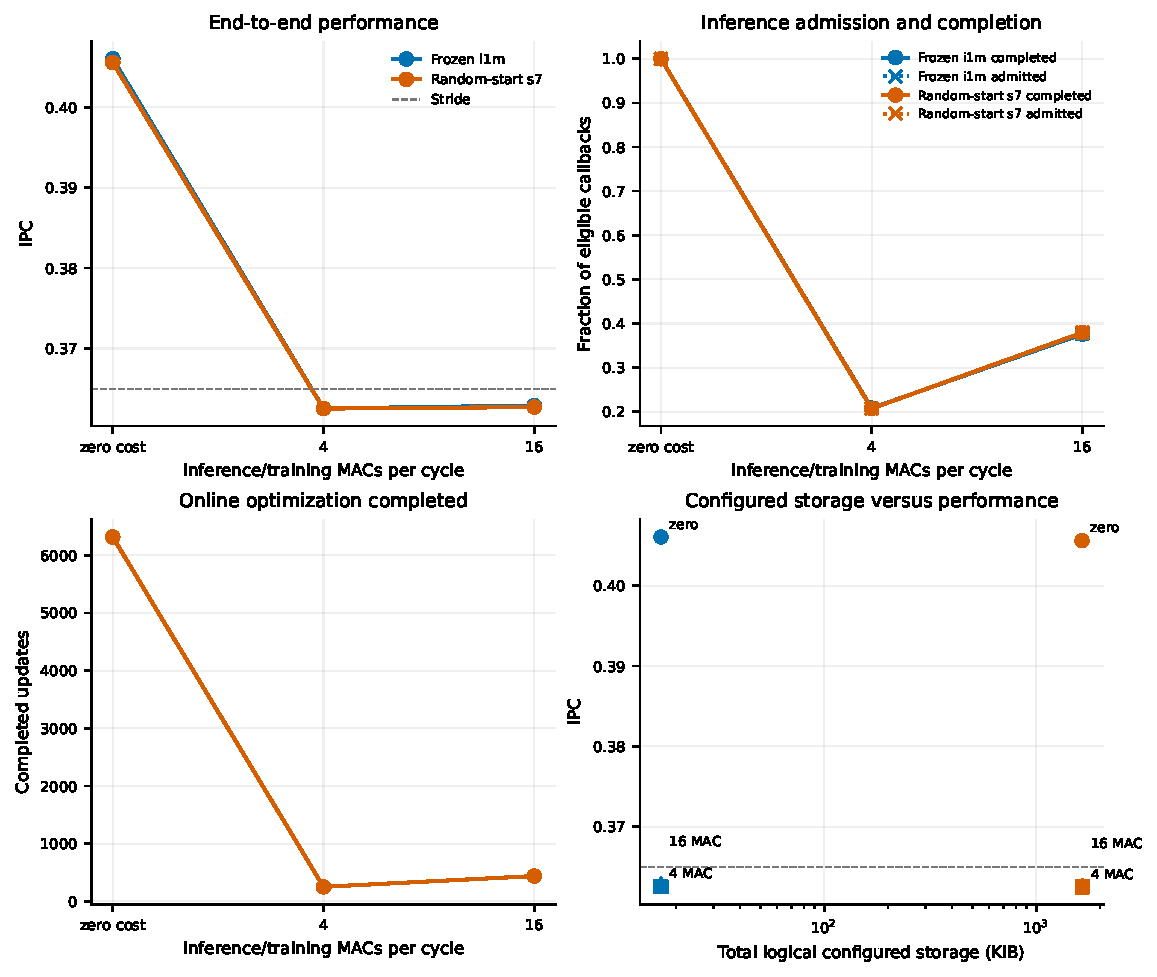
\includegraphics[width=0.98\linewidth]{figures/figure_20_finite_sensitivity.pdf}
\caption{Measured h8 seed-7 sensitivity with the same 64-entry state table and bounded queues. Zero cost isolates finite capacity; 4 and 16 MACs/cycle add the predeclared inference, training and publication service model. Log storage axis compares configured logical FP32 storage, including the online trainer. Service costs are architectural assumptions, not measured silicon.}
\end{figure}

\begin{figure}[p]
\centering
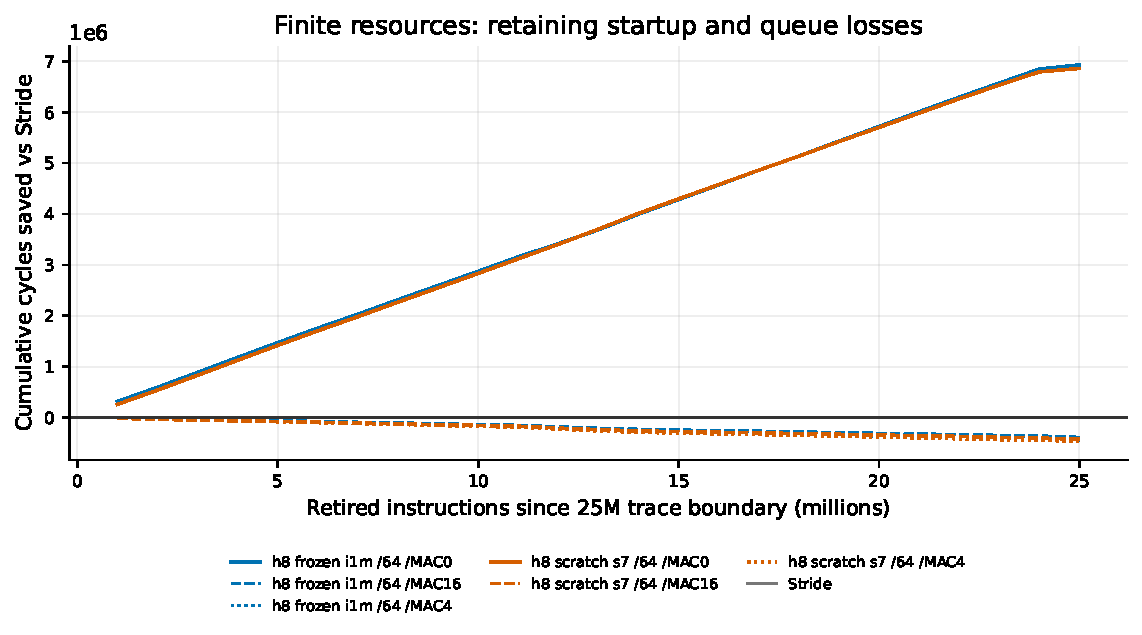
\includegraphics[width=0.92\linewidth]{figures/figure_21_cumulative_cycles_saved_vs_stride.pdf}
\caption{Each finite arm uses its own live closed-loop callback order. Solid, dotted and dashed lines denote zero cost, 4 MACs/cycle and 16 MACs/cycle respectively; color distinguishes frozen and scratch. The matched conventional Stride reference is shared only within the cold-start protocol.}
\end{figure}

\begin{center}
\small
\begin{longtable}{lrrrr}
\toprule
Finite h8 design & MACs/cycle & IPC & Cycles (M) & Saved vs Stride (M) \\
\midrule
\endhead
h8 frozen i1m /64 /MAC0 & 0 & 0.40606 & 61.567 & 6.931 \\
h8 frozen i1m /64 /MAC16 & 16 & 0.36290 & 68.889 & -0.392 \\
h8 frozen i1m /64 /MAC4 & 4 & 0.36254 & 68.958 & -0.460 \\
h8 scratch s7 /64 /MAC0 & 0 & 0.40560 & 61.637 & 6.860 \\
h8 scratch s7 /64 /MAC16 & 16 & 0.36271 & 68.926 & -0.428 \\
h8 scratch s7 /64 /MAC4 & 4 & 0.36252 & 68.961 & -0.463 \\
\bottomrule
\end{longtable}
\end{center}

\begin{center}
\scriptsize
\begin{longtable}{lrrrrrr}
\toprule
Finite design & Eligible & Completed NN & Input drops & Training drops & Updates & State evictions \\
\midrule
\endhead
h8 frozen i1m /64 /MAC0 & 404,271 & 404,271 & 0 & 0 & 0 & 30 \\
h8 frozen i1m /64 /MAC16 & 404,271 & 152,062 & 252,192 & 0 & 0 & 0 \\
h8 frozen i1m /64 /MAC4 & 404,271 & 84,091 & 320,163 & 0 & 0 & 0 \\
h8 scratch s7 /64 /MAC0 & 404,271 & 404,271 & 0 & 0 & 6,316 & 30 \\
h8 scratch s7 /64 /MAC16 & 404,271 & 153,309 & 250,945 & 125,021 & 440 & 0 \\
h8 scratch s7 /64 /MAC4 & 404,271 & 83,740 & 320,514 & 67,420 & 253 & 0 \\
\bottomrule
\end{longtable}
\end{center}

\begin{center}
\scriptsize
\begin{longtable}{llrrr}
\toprule
Finite online design & Milestone & First M & Confirm M & Updates at first \\
\midrule
\endhead
h8 scratch s7 /64 /MAC0 & Saved cycles & 1.0 & 3.0 & 253 \\
h8 scratch s7 /64 /MAC0 & 99\% finite frozen & 2.0 & 4.0 & 505 \\
h8 scratch s7 /64 /MAC16 & Saved cycles & NOT REACHED & NA & NA \\
h8 scratch s7 /64 /MAC16 & 99\% finite frozen & 1.0 & 3.0 & 17 \\
h8 scratch s7 /64 /MAC4 & Saved cycles & NOT REACHED & NA & NA \\
h8 scratch s7 /64 /MAC4 & 99\% finite frozen & 1.0 & 3.0 & 9 \\
\bottomrule
\end{longtable}
\end{center}

h8 frozen i1m /64 /MAC0: IPC was 100.00\% of its unbounded zero-cost control, with 290 additional end-to-end cycles. Completed inference covered 100.00\% of eligible callbacks, with 0 input drops and 0 training drops. It finished with 0 queued inputs, 0 inference job, 0 pending training decisions, and 0 update in flight. This separates capacity loss from modeled service congestion.

h8 frozen i1m /64 /MAC16: IPC was 89.37\% of its 64-entry zero-cost control, with 7,322,790 additional end-to-end cycles. Completed inference covered 37.61\% of eligible callbacks, with 252,192 input drops and 0 training drops. It finished with 16 queued inputs, 1 inference job, 0 pending training decisions, and 0 update in flight. This separates capacity loss from modeled service congestion.

h8 frozen i1m /64 /MAC4: IPC was 89.28\% of its 64-entry zero-cost control, with 7,391,367 additional end-to-end cycles. Completed inference covered 20.80\% of eligible callbacks, with 320,163 input drops and 0 training drops. It finished with 16 queued inputs, 1 inference job, 0 pending training decisions, and 0 update in flight. This separates capacity loss from modeled service congestion.

h8 scratch s7 /64 /MAC0: IPC was 100.00\% of its unbounded zero-cost control, with -208 additional end-to-end cycles. Completed inference covered 100.00\% of eligible callbacks, with 0 input drops and 0 training drops. It finished with 0 queued inputs, 0 inference job, 47 pending training decisions, and 0 update in flight. This separates capacity loss from modeled service congestion.

h8 scratch s7 /64 /MAC16: IPC was 89.43\% of its 64-entry zero-cost control, with 7,288,538 additional end-to-end cycles. Completed inference covered 37.92\% of eligible callbacks, with 250,945 input drops and 125,021 training drops. It finished with 16 queued inputs, 1 inference job, 64 pending training decisions, and 1 update in flight. This separates capacity loss from modeled service congestion.

h8 scratch s7 /64 /MAC4: IPC was 89.38\% of its 64-entry zero-cost control, with 7,323,803 additional end-to-end cycles. Completed inference covered 20.71\% of eligible callbacks, with 320,514 input drops and 67,420 training drops. It finished with 16 queued inputs, 1 inference job, 64 pending training decisions, and 1 update in flight. This separates capacity loss from modeled service congestion.

\begin{center}
\scriptsize
\begin{longtable}{lrrrrr}
\toprule
Finite design & MAC/infer. & Nonlinear/infer. & MAC/update & Nonlinear/update & Weight B/cycle \\
\midrule
\endhead
h8 frozen i1m /64 /MAC0 & 1,825.8 & 78.6 & NA & NA & 0.0 \\
h8 frozen i1m /64 /MAC16 & 1,801.6 & 75.9 & NA & NA & 64.0 \\
h8 frozen i1m /64 /MAC4 & 1,801.1 & 75.9 & NA & NA & 16.0 \\
h8 scratch s7 /64 /MAC0 & 1,799.7 & 75.7 & 449,658.1 & 23,754.2 & 0.0 \\
h8 scratch s7 /64 /MAC16 & 1,794.8 & 75.2 & 531,477.0 & 24,410.1 & 64.0 \\
h8 scratch s7 /64 /MAC4 & 1,805.6 & 76.4 & 562,409.0 & 24,561.9 & 16.0 \\
\bottomrule
\end{longtable}
\end{center}

Across the completed timed arms, 97.85--98.24\% of actual unique PQ enqueues resolved as redundant cache hits: the target line was already resident when the request was serviced. These are not late prefetches under the legacy $L$ counter. Consequently legacy timeliness remained 98.87--99.92\% while useful coverage was only 0.24--0.64\%. The ratio $U/(U+L)$ excludes redundant-cache outcomes; a high value cannot establish useful coverage or a timing-costed win. The issue-cohort outcomes expose this distinction without redefining legacy timeliness.

Per-inference and per-update averages divide work by started jobs. MAC and service-cycle counters charge a full operation at its start, including a final operation that may extend beyond the retirement boundary; these totals are not measured engine utilization. Simulator completed updates and sample exposures advance at modeled training completion, while publication occurs later. A worker may finish an additional host batch during shutdown, so worker diagnostics do not replace the simulator completion/version counters. Raw MAC, nonlinear, state-traffic and publication-cycle totals, queue peaks, drops, and unfinished jobs are in \texttt{resources.csv}.

\subsection{Measured host co-simulation costs}

\begin{center}
\scriptsize
\begin{longtable}{lrrrr}
\toprule
Run & Simulator wall s & Simulator RSS MiB & Worker CPU s & Worker RSS MiB \\
\midrule
\endhead
h16 scratch s17 & 253.01 & 10.99 & 131.65 & 281.98 \\
h16 scratch s27 & 251.43 & 10.75 & 129.63 & 283.96 \\
h16 scratch s7 & 251.38 & 10.79 & 130.40 & 282.27 \\
h8 scratch s17 & 244.53 & 10.46 & 132.24 & 280.20 \\
h8 scratch s27 & 228.15 & 10.55 & 114.71 & 280.23 \\
h8 scratch s7 & 227.02 & 10.50 & 114.15 & 280.38 \\
h8 scratch s7 /64 /MAC0 & 252.51 & 10.91 & 141.62 & 282.89 \\
h8 scratch s7 /64 /MAC16 & 117.52 & 10.50 & 12.67 & 282.59 \\
h8 scratch s7 /64 /MAC4 & 109.18 & 10.53 & 8.25 & 282.09 \\
h16 warm i1m s7 & 253.18 & 10.66 & 131.47 & 282.31 \\
h8 warm i1m s7 & 241.60 & 10.61 & 129.39 & 280.64 \\
\bottomrule
\end{longtable}
\end{center}

RSS includes whole host processes, libraries, allocators and IPC and is not predictor SRAM. Simulator wall time includes waits for the persistent CPU worker. Neither host wall time nor CPU time becomes simulated CPU stalls; congestion is accounted through the declared simulated engines and memory requests.

\clearpage\section{Historical measurements: context, not replacements}

The prior 1M plateau refers to the offline trace-start pretraining budget under a fixed 12-epoch Adam 0.002 recipe, with same-H comparisons to the i20m model. It does not mean an online learner became useful after one million observations. i1m supplied 16,172 eligible training decisions, 2,486 positive decisions and 4,875 action atoms; i20m supplied 325,389, 52,059 and 102,140. Offline updates numbered 228 and 4,404 respectively. Whole-trace PC grouping used there is not a causal online schedule when shared weights change.

Actual completed seed-7 live parity logs exist for all 28 exported prior points. From i1m through i20m, the maximum same-H relative IPC deviations were 0.21747\% for h8 and 0.07318\% for h16, meeting the earlier $\pm0.5\%$ descriptive plateau rule. Request pressure and act rates still varied by roughly 13--15\%; policy equivalence was not established. These warm-cache historical results are kept separate from new cold-start IPC.

The new historical compatibility runs match 120 of 120 original-parser fields exactly across 4 same-checkpoint comparisons. These comparisons include raw instruction/cycle/cache/prefetch counts and legacy derived ratios. Exact system-counter agreement does not by itself prove every internal floating-point value is identical; Python/C++ software parity is validated separately.

\begin{center}
\scriptsize
\begin{tabular}{lrrrr}
\toprule
New compatibility model & Fields exact & Instructions & Cycles & Cycle difference \\
\midrule
h16 i1m & 30/30 & 25,000,003 & 61,014,571 & 0 \\
h8 i1m & 30/30 & 25,000,003 & 61,103,980 & 0 \\
h16 i20m & 30/30 & 25,000,003 & 60,983,624 & 0 \\
h8 i20m & 30/30 & 25,000,003 & 61,086,777 & 0 \\
\bottomrule
\end{tabular}
\end{center}

\begin{center}
\scriptsize
\begin{longtable}{llrrrr}
\toprule
Historical model & Transport & IPC & Cycles & Coverage & Pressure \\
\midrule
\endhead
h8 i1m & offline keyed replay & 0.40912 & 61,106,147 & 0.580 & 0.878 \\
h8 i1m & frozen live parity & 0.40914 & 61,103,980 & 0.580 & 0.952 \\
h8 i20m & offline keyed replay & 0.40924 & 61,088,223 & 0.576 & 1.016 \\
h8 i20m & frozen live parity & 0.40925 & 61,086,777 & 0.576 & 1.126 \\
h16 i1m & offline keyed replay & 0.40973 & 61,015,850 & 0.583 & 1.082 \\
h16 i1m & frozen live parity & 0.40974 & 61,014,571 & 0.583 & 1.209 \\
h16 i20m & offline keyed replay & 0.40994 & 60,984,797 & 0.585 & 0.974 \\
h16 i20m & frozen live parity & 0.40995 & 60,983,624 & 0.585 & 1.073 \\
\bottomrule
\end{longtable}
\end{center}

\section{Limitations and interpretation}

The experiment studies one held-out slice of one trace, two compact model capacities, three random-start seeds, and one pretrained seed. The recipe is fixed using the development gap before final evaluation. Progressive updates from already passed final events are allowed; later final measurements do not tune hyperparameters. Functional correctness with weak learning is a valid outcome.

Data scarcity is assessed using supervised observations and positive actions; optimization using actual updates/exposures and model behavior; state churn using evictions; traffic using requests, drops and cache outcomes; timing using queue/service/publication counters. A late-window improvement without cumulative recovery is reported as such. No composite score hides trade-offs, and absent milestones remain NOT REACHED.

The compact committed tables are \path{summary.csv}, \path{windows_1m.csv}, \path{windows_100k.csv}, \path{learning_milestones.csv}, \path{occupancy_milestones.csv}, \path{issue_cohorts.csv}, \path{storage.csv}, and figure inputs. Raw traces, checkpoints, logs, and training buffers remain outside tracked source. Build, test, pilot, run, status, resume, and report commands are in \texttt{command.md}.

\end{document}
